\documentclass[12pt,onecolumn,a4paper,fleqn]{article}
\usepackage{epsfig,graphicx,subfigure,amsthm,amsmath}
\usepackage{fancyhdr}
\usepackage{setspace}
\usepackage{sidecap}
\usepackage{tikz}
\usepackage{pgfplots}
\usetikzlibrary{decorations.pathreplacing}
\usepackage{relsize}
\usepackage{color}
\usepackage{ifthen}
\usepackage[framed,numbered]{matlab-prettifier}
\usepackage{files/persianheader}     
\usepackage{float}
\usepackage{enumerate}
\usepackage{booktabs}
\usepackage{xepersian}


\settextfont[Path=fonts/,BoldFont={ZarBd.ttf},BoldFeatures={Scale=0.9}]{BZar.ttf}
\setdigitfont[Path=fonts/,BoldFont={ZarBd.ttf},BoldFeatures={Scale=0.9}]{BZar.ttf}

\pagestyle{fancy}
\fancyhf{}
\rhead{\textbf{علوم اعصاب یادگیری}}
\chead{\textbf{پروژه‌ی پایانی درس}}
\lhead{\textbf{\nouppercase{\rightmark}}}
\cfoot{({\thepage})}
\renewcommand{\headrulewidth}{1pt}
\renewcommand{\footrulewidth}{1pt}
\renewcommand{\sectionmark}[1]{\markright{#1}}
\renewcommand{\subsectionmark}[1]{\markright{#1}}
\newcommand{\pf}[1]{$\mathtt{#1}$}
\onehalfspacing
\begin{document}
	\relscale{1}
	\neurotitlepage

\section{آشنایی با هدف پژوهش}

\subsection{هدف پژوهش}
هدف این مقاله مدل سازی \lr{receptive field} نورون‌های پیچیده‌ غشر بصری\footnote{\lr{Visual cortex}} می‌باشد. در واقع با اعمال تحریک‌های تصادفی \lr{spatiotemporal} از توزیع 
$p(s)$
و مشاهده‌ی پاسخ نورون‌ها می‌خواهیم راستایی را بدست بیاوریم که در آن $p(s|r)$ تفاوت معناداری با توزیع اولیه‌ی تحریک‌ها داشته باشد.

تفاوت این مقاله با پژوهش‌های قبل خود آن است که به دلیل رفتار غیر-خطی نورون‌های پیچیده‌ی موجود در \lr{Visual cortex}  نمی‌توانیم از آنالیز‌های خطی 
\lr{spike-triggered average}
که پیش از این کارگشا بودند استفاده کنیم. این مقاله روش 
\lr{spike-triggered correlation analyses}
 را پیشنهاد می‌دهد که بر پایه‌ی \lr{Wiener Kernel} طراحی شده است.

نهایتا با این پژوهش با بررسی‌هایی که انجام می‌دهد ادعا می‌کند که می توان  با این روش پایه‌ای برای تحریک‌ها ارائه داد که تعداد کمی از آن‌ها مشخص کننده‌ی ویژگی‌های مرتبط و تعداد زیادی مربوط به ویژگی‌های پوچ می‌باشند.
\subsection{نورون‌های‌ «پیچیده»}
این مفهوم اولین بار در مقاله‌ی نوبلیست \lr{Hubel and Wiesel} مطرح شده است. نورون‌های ساده نورون‌هایی هستند که رابطه‌ی تحریک-پاسخ آنها نسبت به زمان خطی می‌باشد. این موضوع باعث به وجود آمدن مناطق \lr{ON-OFF} در \lr{Receptive Field} نورون مورد نظر می‌شود. به عکس دست نوشته‌ی موجود در مقاله‌ی مذکور برای جزئیات بیشتر توجه کنید.

\begin{figure}[h]
	\centering
	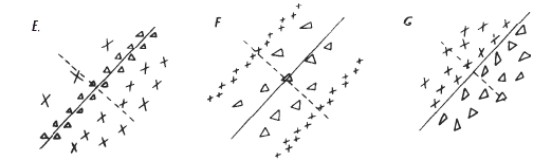
\includegraphics[width=0.8\linewidth]{photos/simple_cells.png}
  \caption[]{مناطق \lr{ON-OFF} حوزه‌ی دریافتی نورون‌های ساده\footnotemark}
\end{figure}
\footnotetext{\lr{EVOLUTION OF IDEAS ON THE PRIMARY
		VISUAL CORTEX, 1955-1978. BY DAVID H. HUBEL}}

همچنین در بخش 
\lr{Material and Methods}
آمده است که اگر نسبت هارمونیک اول به مقدار \lr{DC} حوزه‌ی دریافتی بزرگتر از یک باشد نورون را ساده می‌نامیم. روشن است که نورون‌هایی که از تعاریف بالا پیروی نکنند ساده نبوده و پیچیده‌اند.

\subsection{\lr{STC analysis}}
می‌دانیم که اگر یک ویژگی در تحریک باعث تغییر احتمال اسپایک زدن شود، می‌دانیم که اگه تحریک‌ها را به فضای آن \lr{spike-triggered} منتقل کنیم باید تفاوت قابل توجهی بین مقادیر $p(s|r)$ و $p(s)$ باشد.\footnote{$p(\text{stimulus\ |\ response})$} 

روش‌های مبتنی بر \lr{correlation} با هدف بررسی تغییر این توزیع احتمالات با توجه به تغییرات گشتاور مرتبه‌ی دوم آنها(واریانس) طراحی می‌شوند.

در این بین روش \lr{PCA} به این خاطر که پایه‌ای در اختیار ما قرار می‌دهد که راستا‌های بیشترین تا کمترین واریانس می‌باشند، بسیار مناسب کار ما خواهد بود و می‌تواند ویژگی‌هایی را که در آن واریانس تحریک‌ها بسیار بالا می‌باشد را در اختیار ما بگذارد.

روش \lr{spike-triggered analysis} مبتنی بر موارد فوق مراحل زیر را انجام می‌دهد:
\begin{enumerate}
	\item ابتدا با فرض اینکه حافظه‌ی نورون‌ها بیشتر از ۱۶ فریم یا ۲۶۸ میلی‌ثانیه نخواهد بود؛ پترن‌های تحریک را متشکل از ۱۶ نوار رنگی در ۱۶ فریم و در فضای ۲۵۶ بعدی تعریف می‌کنیم.	
	\item ماتریس \lr{spike-triggered correlation} 
	را به صورت زیر تعریف می‌کنیم:
	$$ C = \frac1N \sum_{i = 1}^{N} S(i)^TS(i) $$
	که در آن $S(i)$ بردار ۲۵۶ بعدی در $i$امین باریست که نورون در طول آزمایش اسپایک زده است و $N$ تعداد کل اسپایک‌ها در طول آزمایش است.
	\item بردارویژه‌ها و مقدارویژه‌های این ماتریس محاسبه شده و با توجه به اندازه‌ی مقدار‌ویژ‌ه‌ها رتبه‌بندی می‌شوند.‌	
\end{enumerate}

با توجه به \lr{PCA} می‌دانیم که حاصل راستا‌هایی خواهد بود که در آن واریانس تحریک‌هایی که موجب اسپایک می‌شوند از زیاد به کم مرتب شده اند.
	
\subsection{اعتبارسنجی نتایج}
برای اعتبارسنجی مشاهدات روش \lr{spike-triggered correlation} روشی که مقاله‌ استفاده می‌کند این است که دنباله‌ای از اسپایک‌های تصادفی با تعداد اسپایک‌های مساوی با $N$ تولید می‌کند و ماتریس \lr{correlation} تحریک‌هایی که موجب این اسپایک‌های فرضی تصادفی شدند را ایجاد می‌کنیم. هدف این است که \lr{control correlation matrix} را محاسبه کنیم که به این معناست که روشی که در قبل پیش گرفتیم را برای داده‌هایی که می‌دانیم مستقل از اسپایک زدن هستند(تمام داده‌ها)نیز اعمال کنیم. با توجه به حجم بالای داده‌ها $N$ مساوی تعداد اسپایک‌ها را در نظر می‌گیریم و ۵ بار فرایند تولید \lr{control correlation matrix} را انجام می‌دهیم و میانگین مقدارویژه‌ها را محاسبه می‌کنیم.با توجه به متن مقاله حاصل این میانگین‌گیری 
$\pm 5.2 SD$ 
بازه‌ی اطمینان ما با $p< 10^{-4}$ خواهد بود. و بنابراین اگر مقدارویژه‌ای خارج از این بازه‌ی اطمینان باشد؛ آن مقدارویژه و بردارویژه دارای تفاوت آشکار خواهند بود.(در واقع آن بردار ویژه راستاییست که تحریک‌های موجب اسپایک در آن واریانس و در نتیجه‌ توزیع احتمال کاملا متفاوتی با توزیع اولیه دارند)
\subsection{نتایج پژوهش}
همانطور که در بخش‌های قبل اشاره کردیم هدف پیدا کردن \lr{eigenvalue}هایی بود که خارج از بازه‌ی اطمینان باشند که آن‌ها به عنوان ویژگی‌های اصلی موجود در \lr{receptive-field} گزارش شود.نتایج مقاله نشان می‌دهد که برای تعداد زیادی از سلول‌های پیچیده دو بردارویژه پیدا شده‌است که این بردار ویژه‌ها ناحیه‌ی \lr{ON-OFF}  مشخص و مجزا ازهمی دارند و همچنین \lr{correlation} بسیار پایینی دارند.همچنین می‌بینیم که این راستا‌ها به خوبی سبب تحریک نورون‌ها می‌شوند با این حال برای \lr{eigenvalue}هایی که در بازه‌ی اطمینان مذکور قرار دارند تاثیر بسیار کمتری در تحریک نورون‌ها مشاهده شده است.

\pagebreak

\section{آشنایی با دیتاست}

\subsection{بخش اول}
با استفاده از تابع تعبیه شده‌ی
	\pf{fget\_hdr.m}
 یکی از فایل‌های \pf{.sa0} را باز می‌کنیم و به محتویات آن توجه می‌کنیم.
 
	\begin{figure}[h]
		\centering
		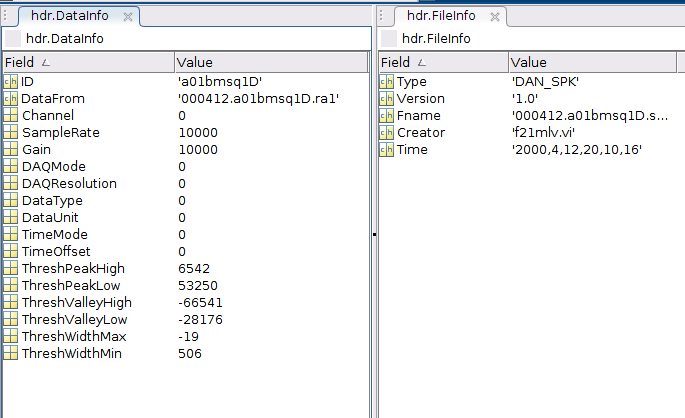
\includegraphics[trim=0.2cm 1cm 0 0.2cm ,clip=true, width=0.8\linewidth]{photos/hdr.png}
		\caption{محتویات فایل \pf{hdr}}
	\end{figure}

می‌توانیم ببینیم که در این فایل اطلاعاتی اطلاعاتی مربوط به خود فایل از جمله‌ زمان ایجاد دیتاست و سازنده‌ی آن و همچنین اطلاعاتی در مورد داده‌ها از جمله نرخ نمونه‌‌گیری وجود دارد.
همچنین در فایل 
\pf{.log} نیز اطلاعاتی مربوط به نورونی که از آن نمونه‌گیری می‌شود وجود دارد.

\begin{table}[h]
	\centering
	\begin{tabular}{|c|c|}
		\hline
		نوع اطلاعات            & برخی از اطلاعات موجود                                \\ \hline
		اطلاعات مربوط به فایل  & زمان ایجاد فایل، سازنده‌ی فایل، ورژن فایل            \\ \hline
		اطلاعات مربوط به تحریک & نوع تحریک، نرخ‌ بروزرسانی مانیتور، نرخ تغییر فریم‌ها \\ \hline
		اطلاعات مربوط به \lr{tuning curve} & زاویه‌‌ی ترجیحی نورون، طول و عرض ترجیحی نورون \\ 
		\hline
				اطلاعات مربوط به نمونه‌‌گیری  & نرخ نمونه‌‌گیری، نوع  کارگذاری الکترود‌ها،  تعداد چنل‌ها         \\ \hline
	\end{tabular}
\end{table}

و اطلاعات دیگری از این دست می‌باشد.

\subsection{بخش دوم}
تابع \pf{Func\_ReadData} را به صورتی که خواسته شده پیاده‌سازی می‌کنیم. ایده‌ی کلی در پیاده‌سازی این تابع این بود که ابتدا با استفاده از تابع \pf{dir} فایل‌های موجود در دایرکتوری نورون مورد نظر را می‌خوانیم و فایل‌های با
\pf{mds1d.sa0}
را پیدا می‌کنیم و اطلاعات آن را با استفاده از 
		\pf{fget\_spk.m}
		می‌خوانیم.
		
		همچنین با توجه به اینکه در بخش بعد به \lr{Spike-count rate} احتیاج پیدا می‌کنیم یکی از خروجی‌های \lr{Optional} را برابر با آن تعریف می‌کنیم، برای محاسبه‌ی این مقدار نیز تنها کافیست توجه کنیم که:
		
		$$ \langle r \rangle = \langle \frac{\#spikes}{time} \rangle_{trials}$$
		
		 نهایتا تابع مورد نظر به صورت زیر خواهد بود:
		


\begin{code}{تابع \pf{Func\_ReadData}}
	\begin{latin}
		\begin{lstlisting}[style=Matlab-editor, tabsize=2]
% Recomend: select Data/ and MatlabFucntions/
% directories and add them to matlab PATH
function [Output, spike_count_rate] = Func_ReadData(NeuronCode)
	Path = [pwd, '/Data', '/Spike_and_Log_Files/', NeuronCode];
	Listing = dir(Path);
	Index_Counter = 0;
	events = {};
	hdrs = {};
	frame_rate = 59.72; %Hz
	frame_number = 32767;
	spike_count = [];
	for i = 1:length(Listing)
		if (contains(Listing(i).name, 'msq1d.sa0', 'IgnoreCase', true) && ...
			~contains(Listing(i).name, 'sa0.sub', 'IgnoreCase', true) && ...
			~contains(Listing(i).name, 'sa0.', 'IgnoreCase', true))
			Index_Counter = Index_Counter + 1;
			[events{Index_Counter}, hdrs{Index_Counter}] = fget_spk(Listing(i).name, 'get');
			spike_count(Index_Counter) = length(events{Index_Counter});
		end
	end
	Output = struct('events', events, 'hdr', hdrs);
	spike_count_rate = mean(spike_count) * frame_rate/frame_number;
end
		\end{lstlisting}
	\end{latin}
\end{code}

\subsection{بخش سوم}
در این بخش ابتدا با استفاده از تابع \pf{dir} در پوشه‌ی مربوط به اطلاعات اسپایک‌ها نام تمام نورون‌ها را استخراج می‌کنیم. سپس با پیمایش بر روی‌ آن‌ها و با استفاده از تابعی که در بخش قبل نوشتیم نرخ اسپایک هر نورون را نگهداری می‌کنیم. نهایتا هیستوگرام نرخ‌ اسپایک‌ها به صورت زیر خواهد بود:

\begin{figure}[h]
	\centering
	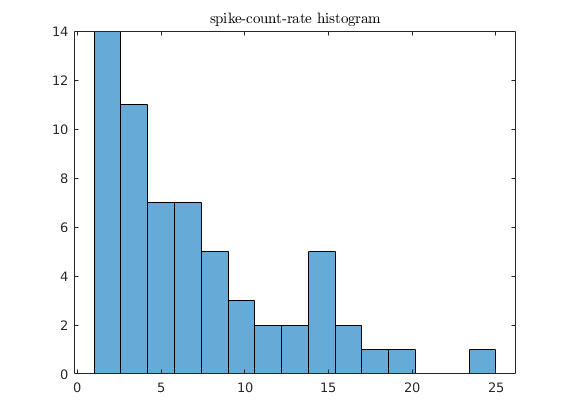
\includegraphics[width=0.6\linewidth]{photos/fr-histogram.png}
	\caption{هیستوگرام نرخ اسپایک‌های نورون‌ها}
	\label{2}
\end{figure}

سپس به سادگی می‌توانیم نورون‌هایی که نرخ اسپایک کمتر از ۲ دارند را با استفاده از قطعه کد زیر از لیست اولیه‌ای که برای کد نورون‌ها تهیه کردیم حذف کنیم.

\begin{code}{حذف نورون‌ها با نرخ اسپایک پایین}
	\begin{latin}
		\begin{lstlisting}[style=Matlab-editor, tabsize=2]
index_counter = 0;
for i = 1:61
	if SCRA(i) < 2
		index_counter = index_counter + 1;
		index(index_counter) = i;
	end
end
fprintf('Exluded Neurons:\n')
disp(neuron_codes(index)')
neuron_codes(index) = [];
		\end{lstlisting}
	\end{latin}
\end{code}


خروجی این قطعه کد شماره‌ی نورون‌های حذف شده را نمایش می‌دهد که به صورت زیر است:
\begin{latin}
	\begin{lstlisting}[basicstyle=\small, frame = single]
Exluded Neurons:
"000413.b03"
"000413.b04"
"000413.b05"
"000418.a01"
"000420.b02"
"000524.c01"
"000907.f07"
	\end{lstlisting}
\end{latin}

\subsection{بخش چهارم}
		در این قسمت تابع \pf{Func\_StimuliExtraction} به گونه‌ای پیاده می‌کنیم که با دریافت دنباله‌ای از زمان اسپایک‌ها تحریک‌هایی با ابعاد 16*16 که سبب این اسپایک‌ها شدند را خروجی بدهد. برای اینکار باید توجه کنیم که با توجه به متن مقاله نرخ تغییر فریم‌های $60Hz$ و به طور دقیق با توجه به فایل‌های لاگ
		 $59.7213Hz$
		 می‌باشد. همچنین از آنجایی که نرخ نمونه برداری $0.1ms$ می‌باشد می‌توان دید که با استفاده از کد زیر می‌تواند اندیس‌هایی از فریم‌ها که در آن‌ها اسپایک رخ‌ داده است را ببینیم.(از آنجایی که تمایل داریم ابعاد ماتریس ۱۶*۱۶ باشد اندیس‌های کمتر از ۱۶ را نادیده در نظر می‌گیریم)

\begin{code}{یافتن اندیس‌های زمان اسپایک و نادیده گرفتن اندیس‌های کمتر ۱۵}
	\begin{latin}
		\begin{lstlisting}[style=Matlab-editor, tabsize=2]
indices = ceil((events * frame_rate) / 10000);
indices = indices(indices>15);
		\end{lstlisting}
	\end{latin}
\end{code}
 
سپس می‌توانیم ماتریس‌های ۱۶*۱۶ که سبب اسپایک شدند را تشکیل دهیم.

برای راحت‌تر شدن کار در مراحل بعد اولا ورودی دوم ذکر شده در صورت سوال یعنی \lr{msq1D} را اختیاری در نظر گرفتیم که مقدار دیفالت آن همان فایلی خواهد بود که در پوشه‌ی \lr{Data} قرار دارد. همچنین در مراحل بعد از آنجایی که می‌خواهیم دنباله‌ای تصادفی از اسپایک‌ها تولید کنیم راحت‌تر خواهد بود که فقط اندیس‌ها را به عنوان ورودی به این تابع بدهیم به این منظور یک ورودی \lr{option} تعریف کردیم که اگر مقدار آن 
\lstinline[style=Matlab-editor, tabsize=2]{'random'}
باشد مقدار \lr{events} در ورودی را به عنوان اندیس‌ها در نظر می‌گیرد و در غیر این صورت همان منطق قبلی را اجرا می‌کند.

\subsection{بخش پنجم}
برای تشخیص مناسب ترین جهت نشان دادن تصاویر، باید آزمایشی ترتیب داده شود که یک ورودی مشخص، در زوایای مختلف به فرد مورد آزمایش نشان داده شود، و نرخ اسپایک زدن متناظر با هر راستا اندازه گیری شود. با شناسایی بیشینه‌ی این نرخ، جهت مناسب پیدا می‌شود.

\begin{figure}[h]
	\centering
	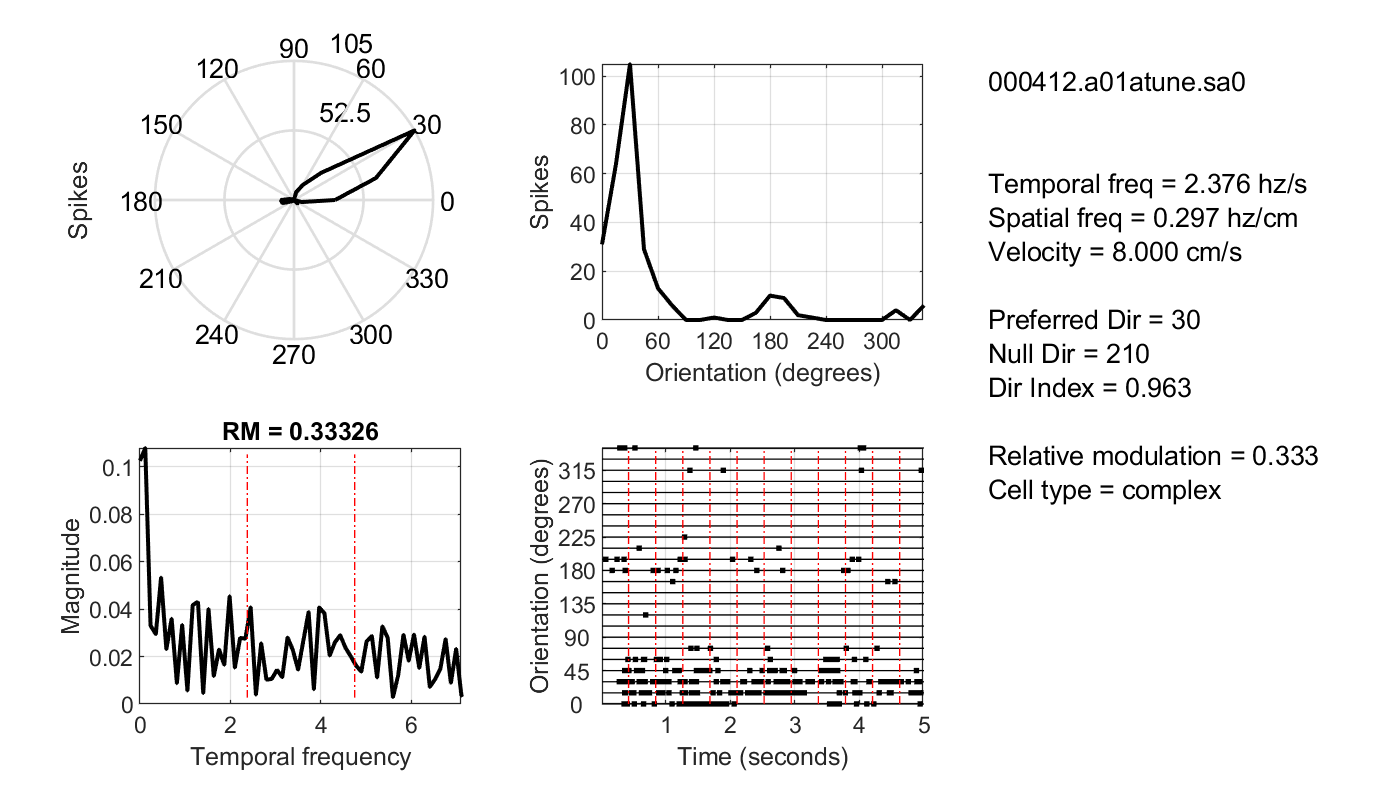
\includegraphics[width=0.85\linewidth]{photos/4_5_000412_a01.png}
	\caption{اطلاعات فایل تیونینگ نورون \lr{000412.a01}}
\end{figure}
		 
\begin{figure}[h]
	\centering
	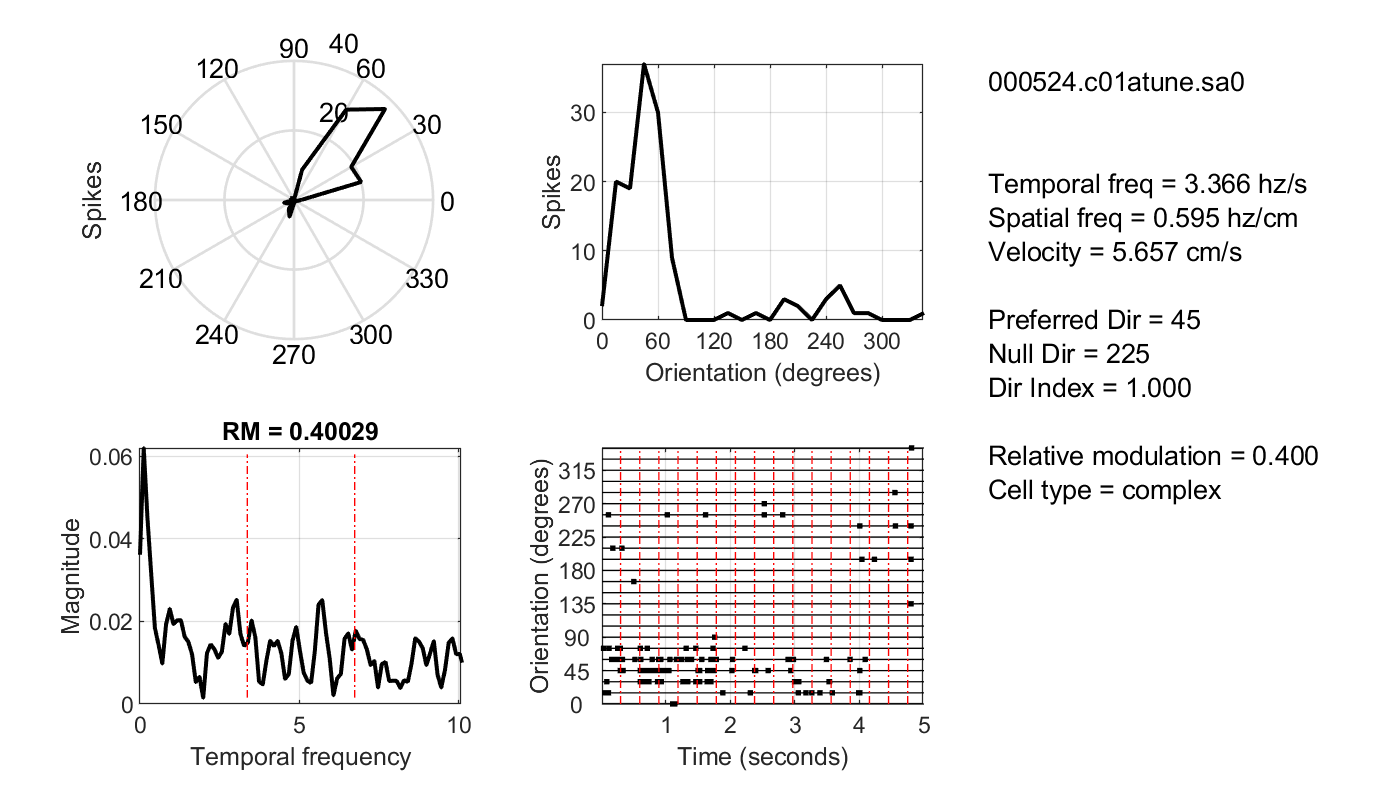
\includegraphics[width=0.85\linewidth]{photos/4_5_000524_c01.png}
	\caption{اطلاعات فایل تیونینگ نورون \lr{000524.c01}}
\end{figure}		 

\pagebreak

\section{بررسی با روش کلاسیک \lr{STA}}

در سکشن دوم کد نهایی که برای این بخش ارائه شده‌ است بر روی تمام ۵۴ نورونی که در بخش قبل حذف نشده‌اند عملیات‌ها صورت می‌گیرد.و حاصل تنها ذخیره می‌شود و تصاویر نمودار‌ها \lr{export} می‌شوند. بنابراین برای تست‌ کردن کد این بخش توصیه می‌شود که ابتدا سکشن اول که مربوط به بارگذاری استراکچر‌های مورد نیاز است را اجرا کرده و سپس از سکشن سوم به بعد که مخصوص تست طراحی شده‌اند را اجرا کنید.
\subsection{بخش اول}
برای محاسبه‌ی این بخش تابع \pf{Func\_FindSTA} پیاده سازی شده است که نحوه‌ی عملکرد آن به صورت زیر است.

\begin{code}{تابع محاسبه‌ی \lr{STA}}
	\begin{latin}
		\begin{lstlisting}[style=Matlab-editor, tabsize=2]
function [sta, spike_trigerred] = Func_FindSTA(neuron)
	outs = neuron.outs;
	spike_trigerred = [];
	for i = 1:length(outs)
spike_trigerred_trial = Func_StimuliExtraction(outs(i).events);
spike_trigerred = cat(3, spike_trigerred, spike_trigerred_trial);
	end
	N = length(spike_trigerred);
	sta = (sum(spike_trigerred, 3)/ N);
end		\end{lstlisting}
	\end{latin}
\end{code}

که می‌توان دید بنابر تعریف \lr{STA} پیاده‌سازی شده است. این تابع تمام مقادیر 
\lstinline[style=Matlab-editor, tabsize=2]{spike_trigerred}
را نیز خروجی می‌دهد چرا که در مراحل بعد به آن نیاز خواهیم داشت. برای همان مثالی که در صورت پروژه آمده است خروجی زیر را می‌گیریم:
\begin{figure}[h]
	\centering
	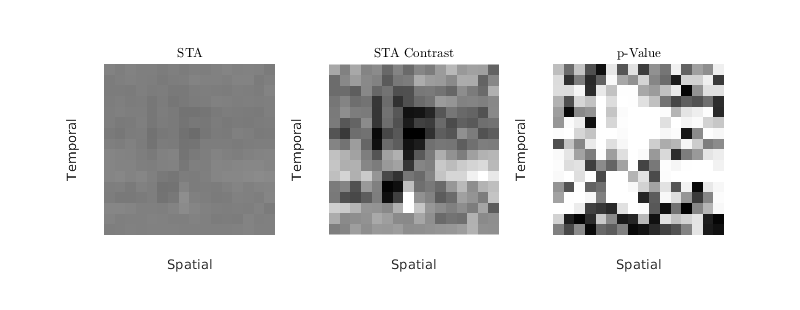
\includegraphics[width=0.5\linewidth]{photos/sta.png}
	\caption{خروجی برای نورون \lr{000601.c05}}
\end{figure}

\subsection{بخش دوم}
خروجی این بخش در بخش اول نمایش داده‌ شد با این حال ذکر می‌کنیم که برای محاسبه‌ی \lr{p-value} به دست آمده از \lr{t-test} از تابع آماده  \pf{ttest}
در متلب استفاده کردیم.
\begin{code}{محاسبه‌ی \lr{t-test}}
	\begin{latin}
		\begin{lstlisting}[style=Matlab-editor, tabsize=2]
[~, p] = ttest(permute(spike_trigerred,[3 1 2]));
	\end{lstlisting}
	\end{latin}
\end{code}

\subsection{بخش سوم}
برای محاسبه‌ی \lr{correlation} از آنجایی که یکی از ماتریس‌هایی که در اختیار ماست ۳بعدی است محاسبه‌ی \lr{correlation} را به صورت دستی انجام دادیم و تابع 
\pf{Func\_Correlation}
را پیاده‌سازی کردیم، که اساس کار آن ضرب درایه به درایه موجود در متلب می‌باشد. همچنین برای تولید دنباله‌ی تصادفی از اسپایک‌ها یا همان ماتریس کنترل به صورت زیر عمل کردیم و در اینجا اضافه کردن پارامتر ورودی اضافه به تابع کارمان را ساده‌تر می‌کند. و تنها کافیست دنباله‌ای تصادفی از شماره‌ی فریم‌ها ایجاد کنیم.
\begin{code}{ایجاد دنباله‌ی تصادفی از تحریک‌ها}
	\begin{latin}
		\begin{lstlisting}[style=Matlab-editor, tabsize=2]
spike_sample = randi([16 32767], 1, N);
stim_control = Func_StimuliExtraction(spike_sample, 'random');
		\end{lstlisting}
	\end{latin}
\end{code}
خروجی هریک از ماتریس‌های کنترل و \lr{spike-triggered} در فضای جدید برای این نورون به صورت زیر است.
\begin{figure}[h]
	\centering
	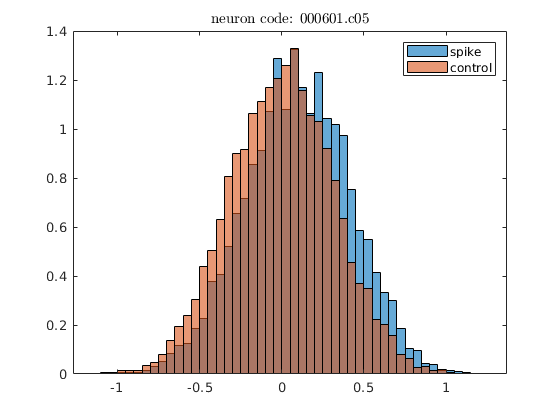
\includegraphics[width=0.46\linewidth]{photos/sta-kernel-hist.png}
	\caption{
		هیستوگرام \lr{correlation} ماتریس‌های کنترل و \lr{spike-triggered} با \lr{STA}
	}
\label{1}
\end{figure}

\subsection{بخش چهارم}
برای محاسبه‌ی \lr{p-value} در اینجا نیز از تابع آماده \pf{ttest2} موجود در متلب استفاده می‌کنیم. خروجی آن به صورت زیر است.

\begin{latin}
	\begin{lstlisting}[basicstyle=\small, frame = single]
p-value = 0.000000, null-hypothesis rejected, means are diffrent.
	\end{lstlisting}
\end{latin}
نتیجه‌ی آزمون \lr{t-test} این است که توزیع‌ $p(s|r)$ و $p(s)$ در فضای مربوط به \lr{STA} دارای میانگین‌های متفاوتی می‌باشند. با این حال با توجه به \autoref{1} برایمان روشن است که این دو توزیع علارغم اینکه میانگین‌های متفاوتی دارند اما به دلیل اینکه‌ سطح مشترک زیر نمودار آنها بسیار زیاد است نمی‌توان تفاوت معناداری بین آنها قائل شد.

به عبارت دیگر نتیجه‌ی آزمون می‌گوید که توزیع‌ $p(s|r)$ و $p(s)$ تفاوت میانگین قابل توجهی دارند که این بر خلاف انتظار ما نمی‌باشد چرا که $p(s|r)$ از تصویر بردارهای منجر به اسپایک بر روی \lr{STA} حاصل می‌شود که واضح است که باید میانگین مثبتی داشته باشد و از طرفی روشن است که با انتخاب تحریک‌های رندم و تصویر کردن روی \lr{STA} میانگینی نزدیک به صفر خواهیم داشت.

با این حال همانطور که از شکل مشخص است تفاوت معنادار در \textbf{میانگین} نمی‌تواند تفاوت معنادار در \textbf{توزیع‌ها} را نشان بدهد و همانطور که از متن مقاله به یاد داریم در آنالیزهایی که بر پایه‌ی \lr{correlation} طراحی می‌شوند تغییر در توزیع‌ها را با تغییر در گشتاور درجه‌ی دوم آنها یا همان واریانس می‌سنجیم.

\subsection{بخش پنجم}
به طور کلی میدانیم که خطای تخمین ما از رابطه‌ی زیر محاسبه می‌شود:
$$ P(\text{Error}) = P(\text{Error}|s=1)P(r=1) + P(\text{Error}|r=0)P(r=0) $$

از طرفی می‌دانیم که با توجه به اینکه تحریک‌های اولیه‌ کاملا تصادفی بودند  $P(s=1)$ همان نرخ اسپایک زدن هر نورون در همین آزمایش می‌باشد. ما قبلا نرخ \lr{spike-count rate} را محاسبه کرده بودیم و از توضیحات درس به یاد داریم که:
$$ P(r=1) = \dfrac{\langle count \rangle}{\Delta t} $$ 
که در اینجا $\Delta t$ همان نرخ تغییر فریم‌ها می‌باشد. حال با توجه به نوع تخمینمان که تنها به یک پارامتر $\theta$ وابسته می‌باشد مقدار خطا را باز نویسی می‌کنیم:

$$ P(\text{Error}) = P(X > \theta | r = 0)P(r = 0) + P(X < \theta | r = 1)P(r = 1) $$

توزیع $P(X|r=1)$ همان توزیع تصویر \lr{spike-triggered } ها بر روی \lr{STA} می‌باشد که طبق فرض مسئله آن را نرمال در نظر می‌گیریم. از طرف دیگر با توجه به \lr{sparse} بودن نورون‌ها و احتمال پایین اسپایک زدن آنها(برای اکثر نورون‌ها با توجه به \autoref{2} در حدود $10^{-2}$ می‌باشند) می‌توانیم توزیعی که برای تصویر \lr{control} محاسبه کردیم را توزیع $P(X|r=0)$ در نظر بگیریم و بنابراین می‌توانیم $P(\text{Error})$ را محاسبه کنیم و مشتق آن نسبت $\theta$ را برابر با صفر قرار دهیم تا بهترین ترشهولد را محاسبه کنیم.

برای محاسبه این مقادیر در متلب ابتدا یک فیت گاوسی بر روی هیستوگرام‌ها ایجاد می‌کنیم و سپس $\mu$ و $\sigma$ را محاسبه می‌کنیم و آن‌ها را به همراه احتمال اسپایک زدن نورون به تابع نوشته شده‌ی
 \pf{Func\_Accuracy} می‌دهیم که ترشهولد و دقت تخمین ما را بیان می‌کند.

\begin{figure}[h]
	\centering
	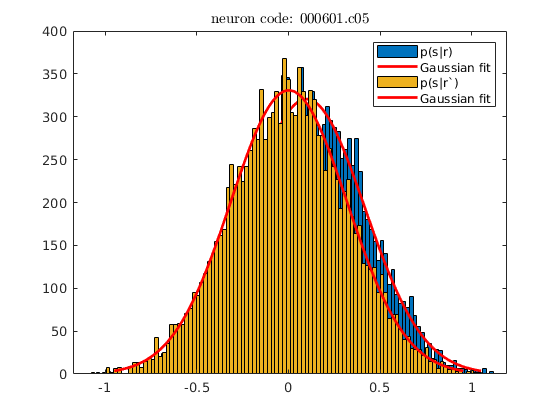
\includegraphics[width=0.6\linewidth]{photos/sta-fit-gaussian.png}
	\caption{
هیستوگرام‌ها به همراه فیت گوسی آن‌ها
	}
	\label{1}
\end{figure}

همچنین توجه می‌کنیم که برای محاسبه‌ی 
\pf{Func\_Accuracy}
از سایت‌های محاسبه کننده استفاده کردیم و خروجی آنها را در تابع متلب قرار دادیم.
 
\pagebreak
		 
		 \subsection{بخش ششم}
		 با اجرای مراحل بالا برای تمامی ۵۴ نورون باقی مانده به خروجی‌های زیر دست پیدا می‌کنیم لازم است توجه کنیم که داده‌های کنترل به صورت رندم تولید می‌شوند و بنابراین با اجرای این کدها ممکن است نتایج اندکی متفاوت بگیریم هر چند در کلیت پاسخ تاثیری نخواهند داشت.
		 \newcounter{int}
		 \setcounter{int}{1}
		 \loop
		 
		 \begin{figure}[ht]
		 	\centering
			\subfigure{\includegraphics[width=0.55\linewidth]{photos/STA/imshows/\theint.png}}
			\hfill
			\subfigure{\includegraphics[width=0.4\linewidth]{photos/STA/histograms/\theint.png}}
		 \end{figure}
		 
		 \addtocounter{int}{1}\ifnum\value{int}<10
		 \repeat
		 
		 
		 \loop
		 
		 \begin{figure}[h]
		 	\centering
		 	\subfigure{\includegraphics[width=0.55\linewidth]{photos/STA/imshows/\theint.png}}
		 	\hfill
		 	\subfigure{\includegraphics[width=0.4\linewidth]{photos/STA/histograms/\theint.png}}
		 \end{figure}
		 
		 
		 \addtocounter{int}{1}\ifnum\value{int}<18
		 \repeat
		 
		 \clearpage
		 
		 \loop
		 
		 
		 \begin{figure}[h]
		 	\centering
		 	\subfigure{\includegraphics[width=0.55\linewidth]{photos/STA/imshows/\theint.png}}
		 	\hfill
		 	\subfigure{\includegraphics[width=0.4\linewidth]{photos/STA/histograms/\theint.png}}
		 \end{figure}	 	     

		 
		 \addtocounter{int}{1}\ifnum\value{int}<55
		 \repeat 
		 
		 \clearpage
		 
		\subsection{بخش هفتم}
	با اینکه میانگین توزیع‌ها با توجه به تست‌های آماری با هم تفاوت دارند از آنجایی که تقریبا تمامی نمودار‌های رسم شده نشان می‌دهند که توزیع تصویر تحریک‌ها بر راستای \lr{STA} برای کلیه تحریک‌ها و تحریک‌هایی که موجب اسپایک شدند تفاوت چشمگیری با هم ندارند و به درستی نمی‌توان ترشهولدی پیدا کرد که با انتخاب آن داده‌ها را با دقت خوبی بتوان دسته‌بندی کرد.از طرف دیگر مولفه‌ی \lr{STA} در بیشتر نورون‌ها الگوی‌ معناداری ندارد و بیشتر شبیه نویز‌ می‌باشد.به عبارتی تا حد خیلی زیادی می‌توان به اعای مقاله مبنی بر پیچیدگی نور‌ون‌هایی که با آنها سروکار داریم استناد کرد.
	
	با این وجود می‌توان دید که برخی از نورون‌های جدولی که در بالا ارائه کردیم نه تنها پترنی با الگوی معنادار دارند بلکه نمودار توزیع آن‌ها به علت تفاوت \textbf{میانگین} که باهم دارند را به خوبی می‌توان تفکیک کرد که نسبت به پیچیده بودن رفتار این دسته از نورون‌ها می‌توان تردید داشت. از بین می‌توان نورون با کد \lr{010718.B.c} را مثال زد به نمودار و نتایج به دست آمده از آن توجه می‌کنیم.
		
	
 \begin{figure}[ht]
 	\centering
 	\subfigure{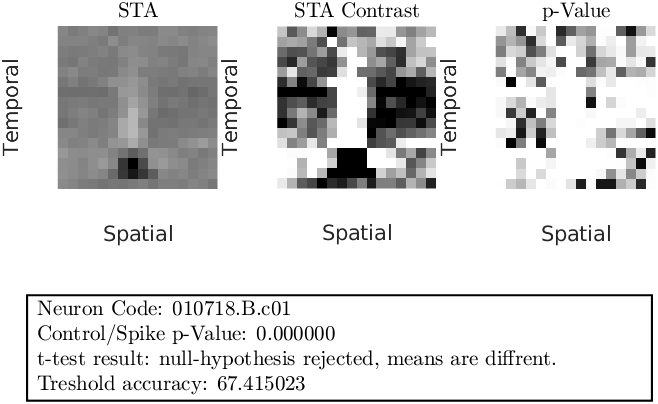
\includegraphics[width=0.55\linewidth]{photos/STA/imshows/37.png}}
 	\hfill
 	\subfigure{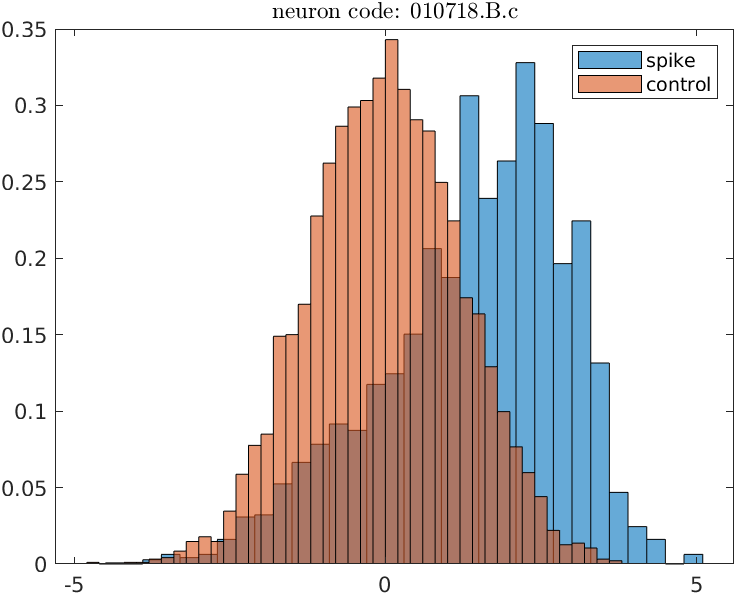
\includegraphics[width=0.4\linewidth]{photos/STA/histograms/37.png}}
 \end{figure}

می‌توانیم ببینیم که دو توزیع آن نسبتا جدایی پذیر به نظر می‌آیند و همچنین الگو معناداری در تصویر با کانتراست بالای \lr{STA} وجود دارد. البه باید توجه کنیم علت اینکه ترشهولد مناسب برای این نورون انتخاب نشده این است که توزیع \lr{spike} در آن گاوسی به نظر نمی‌رسد و فیت گاوسی ما اطلاعات نادرستی از توزیع به ما می‌دهد. به این فیت و داده‌های حذف شده توسط آن توجه کنید.
	 \begin{figure}[ht]
		\centering
		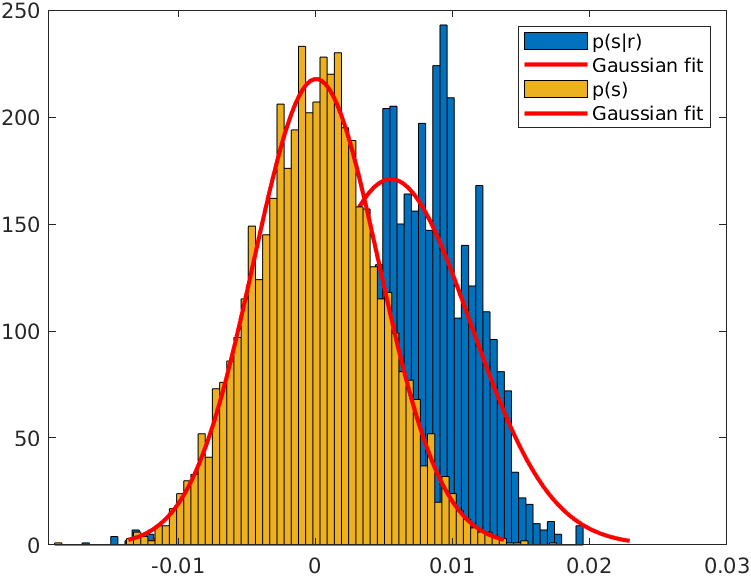
\includegraphics[width=0.4\linewidth]{photos/STA/gaussianFits/37.png}
	\end{figure}

در بین نورون‌های بررسی شده اما نورون‌های دیگری هم وجود داشتند که می‌شد الگوی معنا‌داری در \lr{STA} آنها مشاهده کرد و از این بین می‌شود به نورون	\lr{011025.A.d} اشاره کرد که توزیع‌ نمودار‌های آن هم جدا از هم به نظر می‌رسد.

 \begin{figure}[ht]
	\centering
	\subfigure{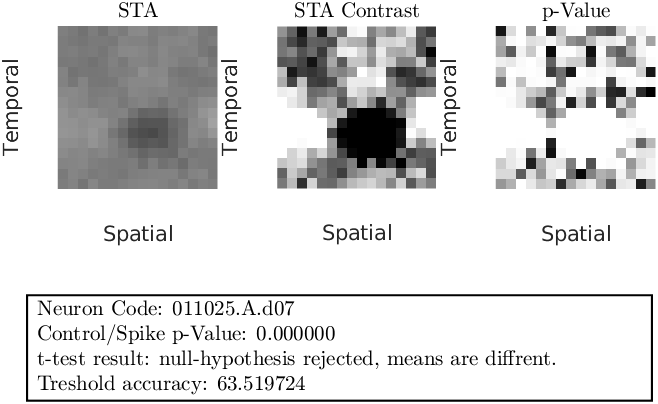
\includegraphics[width=0.55\linewidth]{photos/STA/imshows/42.png}}
	\hfill
	\subfigure{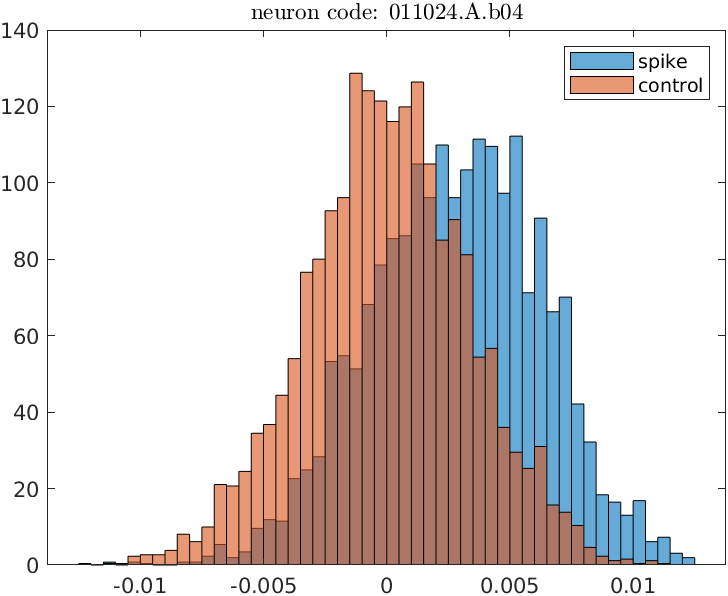
\includegraphics[width=0.4\linewidth]{photos/STA/histograms/42.png}}
\end{figure}

همچنین ترشهولدی که برای این نورون‌ پیدا کردیم درصد قابل توجهی از فریم‌های منجر به اسپایک را شناسایی کرده است.

نهایتا می‌توان گفت به طور کلی ادعای مقاله درباره‌ی پیچیده بودن این نورون‌ها درست به نظر می‌رسد با این حال در مورد تعدادی از آنها باید احتیاط بیشتری به خرج بدهیم.


\pagebreak

\section{ بررسی با روش \lr{Spike-Triggered Correlation}}

در این بخش، از نورون شماره 10 با نام 
\lr{c05.000601}
استفاده شده است.

\subsection{بخش اول}

\begin{figure}[ht]
	\centering
	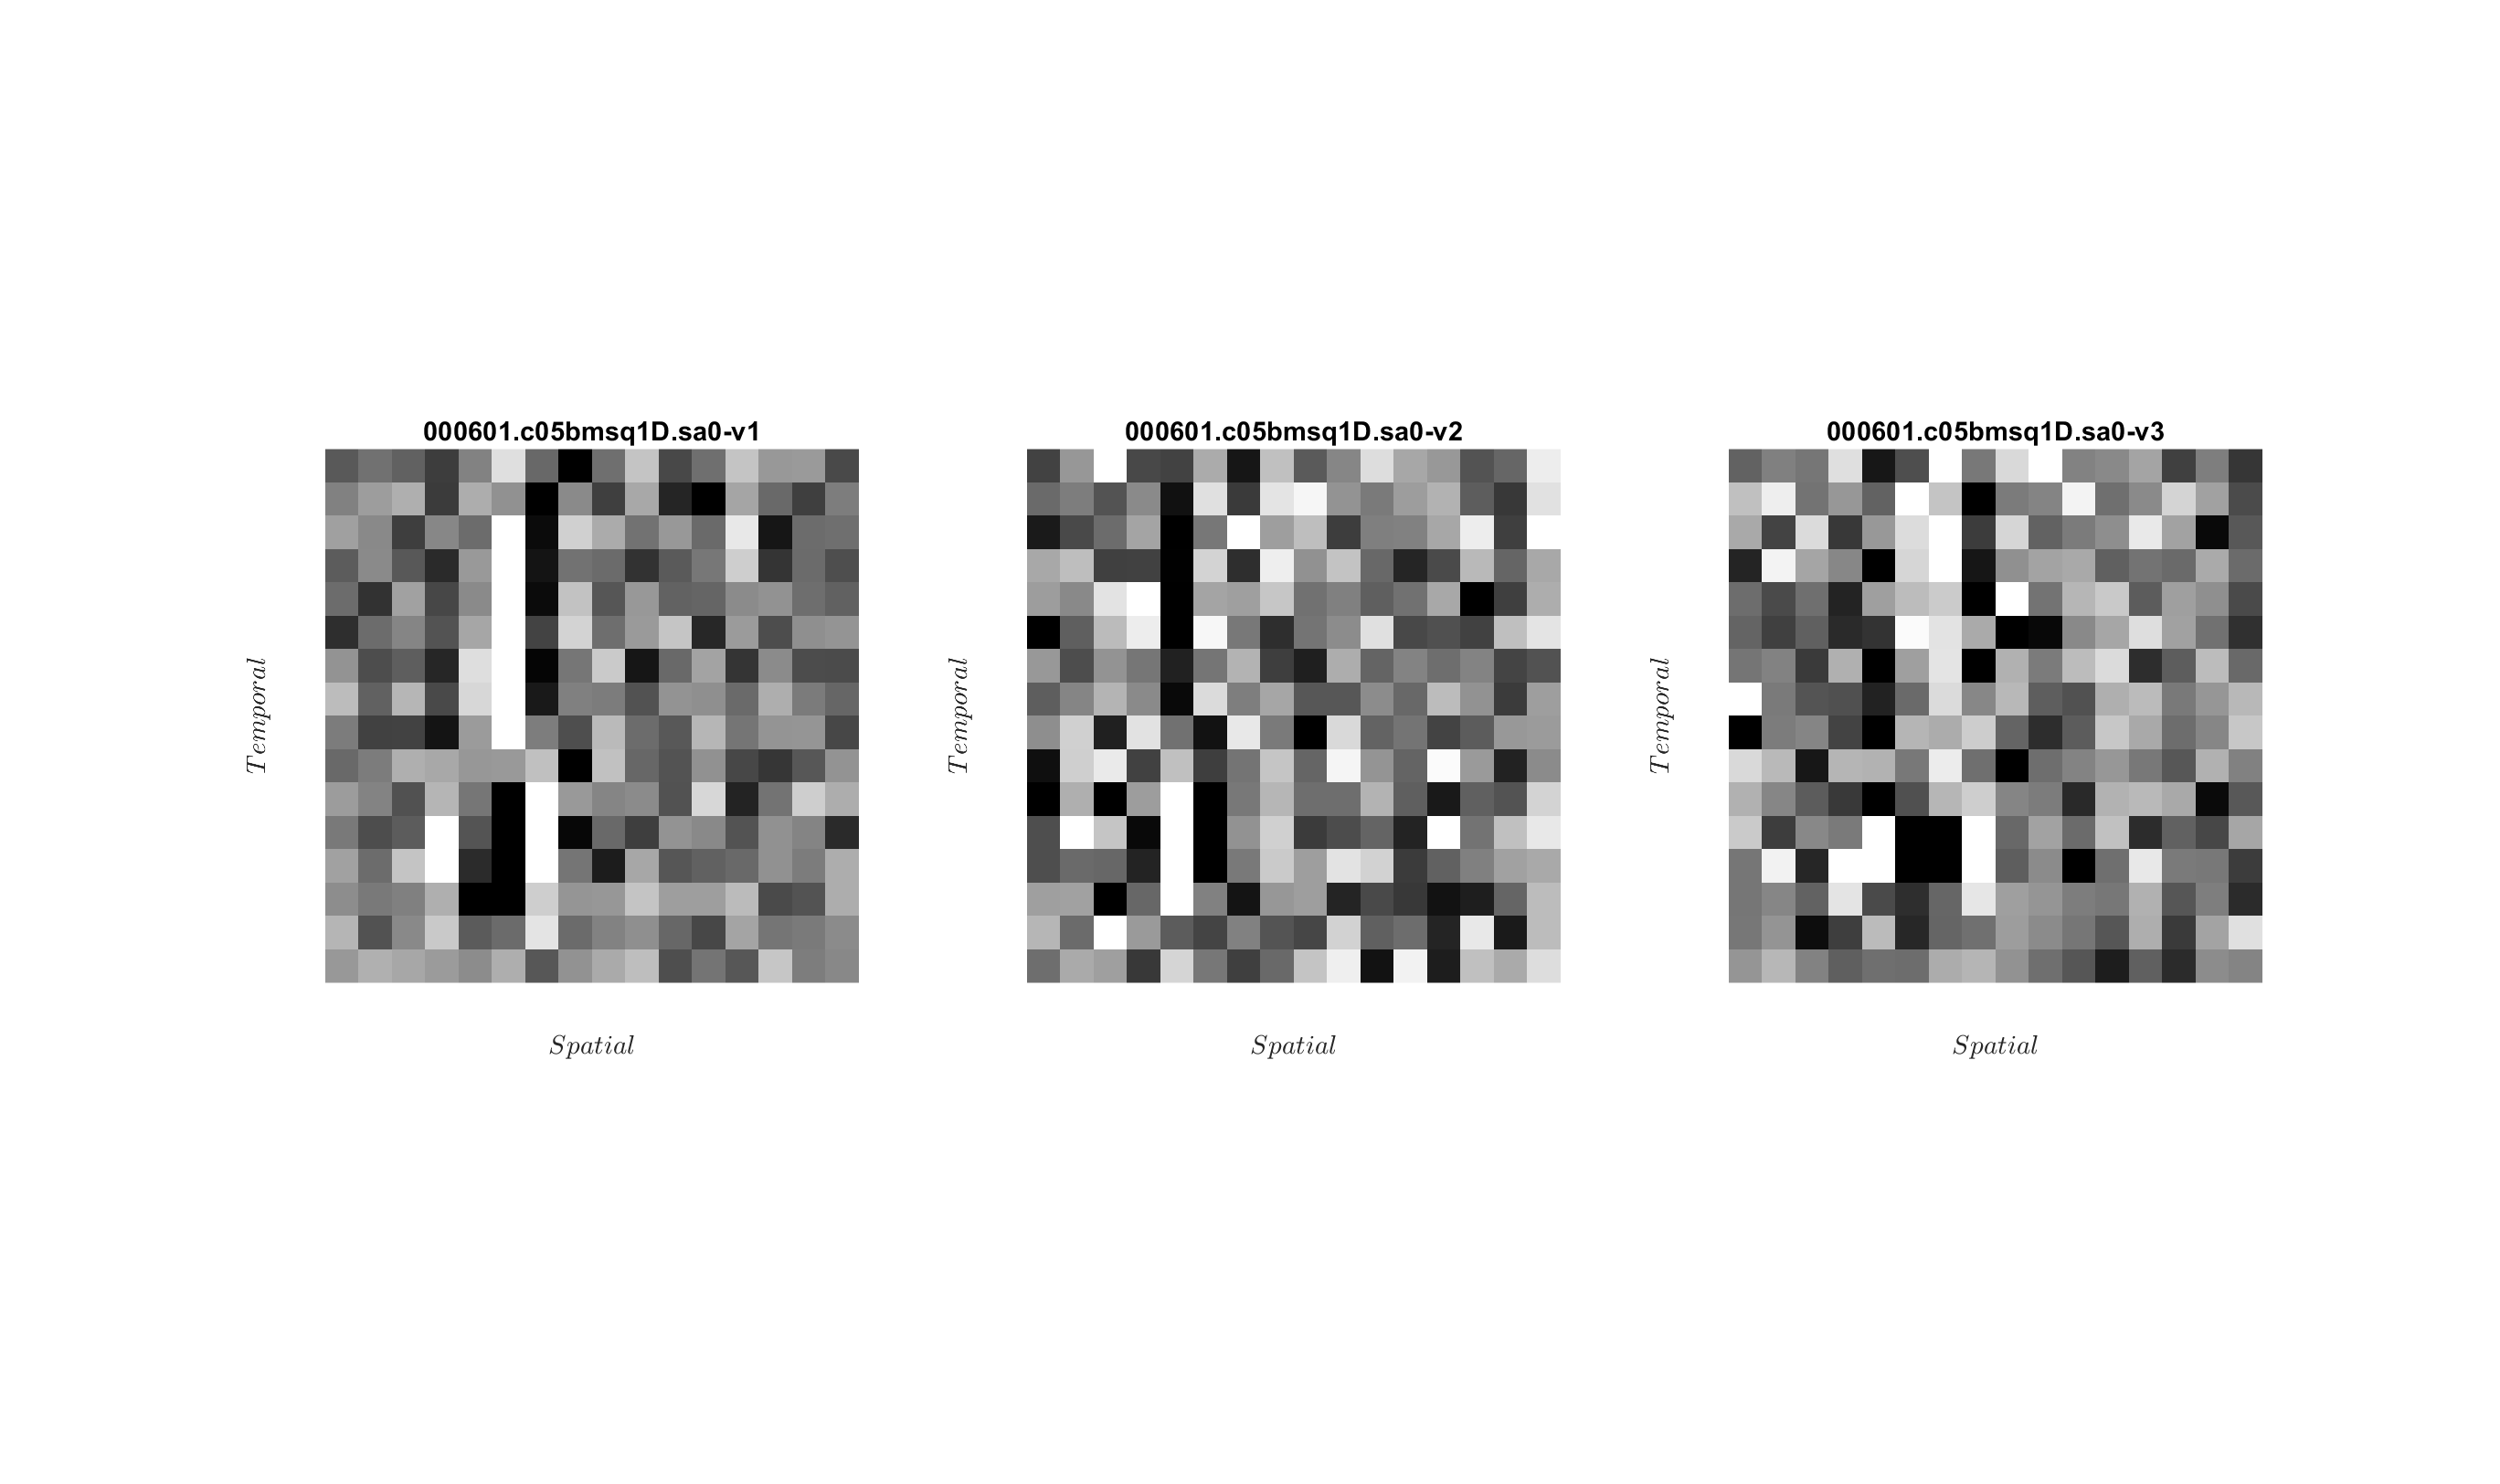
\includegraphics[trim = 5cm 10cm 5cm 10cm, clip= true, width=0.6\linewidth]{photos/4_1.png}
	\caption{بردار ویژه‌های اول تا سوم}
\end{figure}

\subsection{بخش دوم}

\begin{figure}[ht]
	\centering
	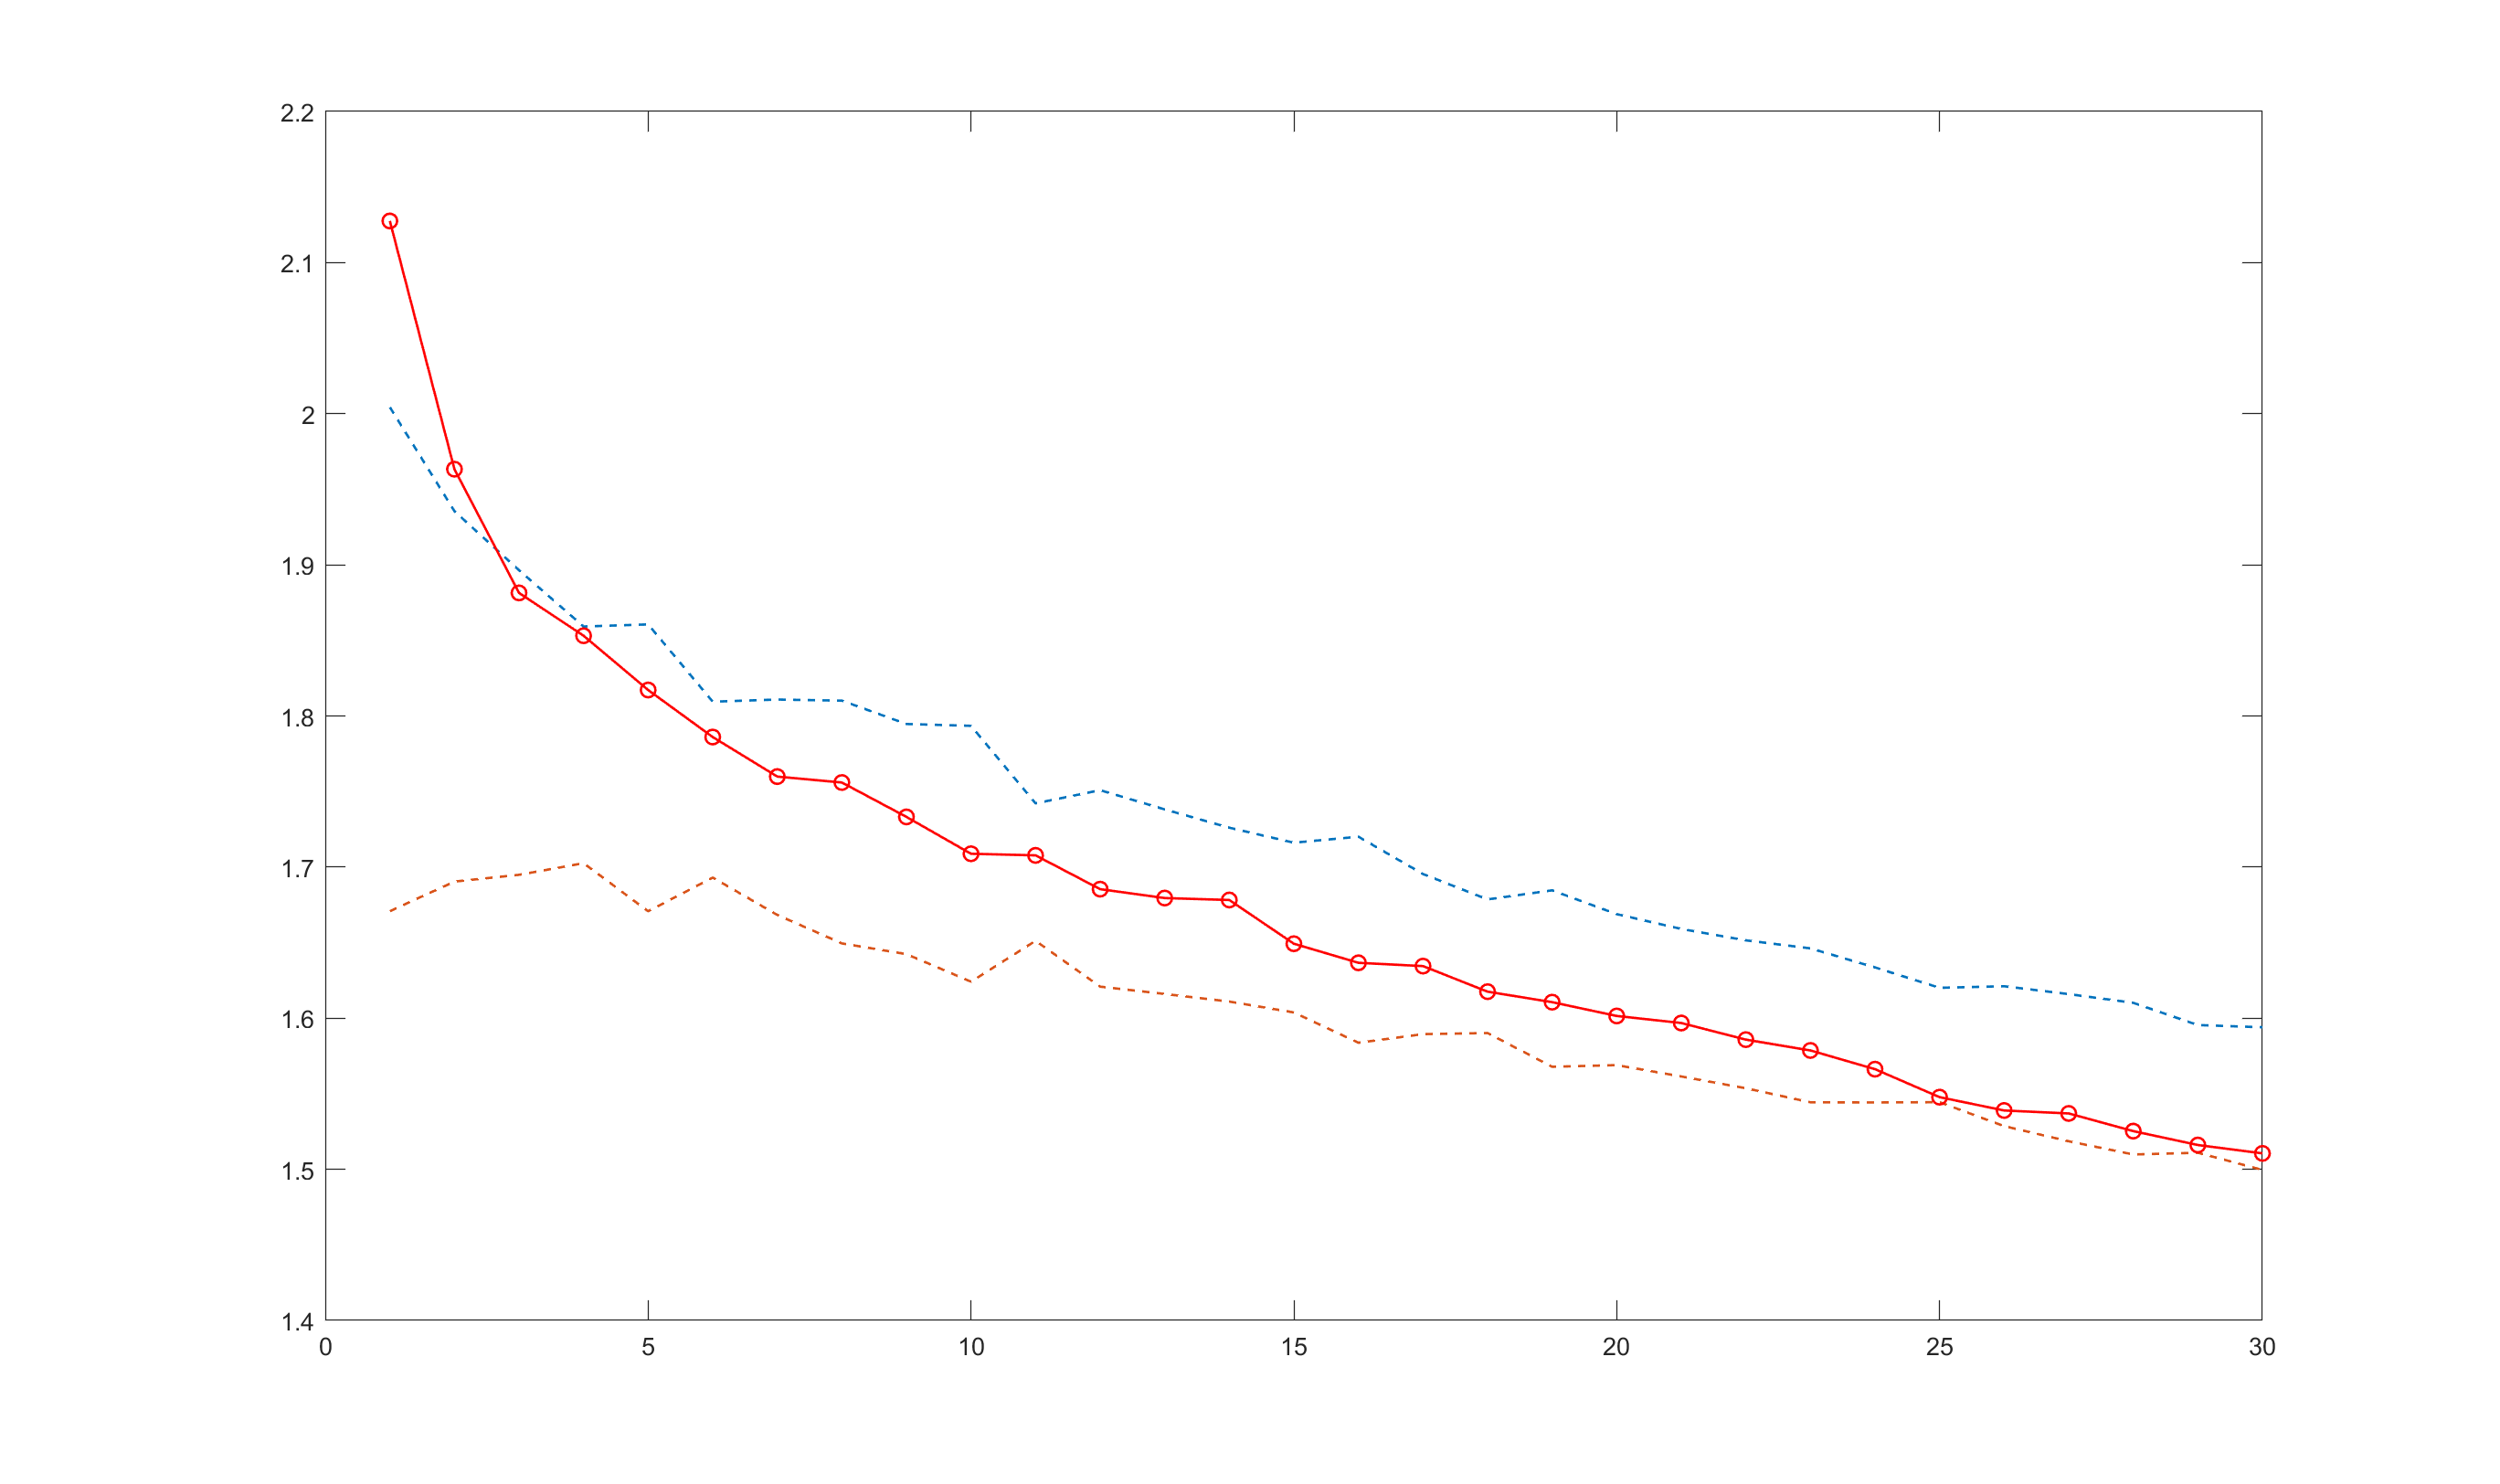
\includegraphics[width=0.6\linewidth]{photos/4_2.png}
	\caption{مقدار ویژه‌ها در کنار بازه‌ی اطمینان }
\end{figure}
برای به دست آوردن بازه های اطمینان مربوط به هر نورون، به روش زیر عمل کردیم:

به تعداد زمان های اسپایک زدن نورون اصلی، زمان تصادفی با توزیع یکنواخت تولید کردیم و این کار را ۲۰ مرتبه انجام دادیم. با استفاده از تابع \pf{Func\_StimuliExtraction }، تحریک‌های متناظر با هر دنباله زمانی را به دست آوردیم. بنابراین در نهایت ۲۰ دنباله تصادفی اسپایک به دست آوردیم که از هر کدام، یک ماتریس کوریلیشن تصادفی به دست می‌آید. به محاسبه مقادیر ویژه این ۲۰ ماتریس و مرتب سازی آن هاُ ۲۰ مجموعه ۲۵۶ تایی از مقادیر ویژه به دست آوردیم. سپس برای محاسبه‌ی بازه اطمینان مربوط به مقدار ویژه $ n $ از ماتریس کوریلیشن اصلی، به سراغ مقادیر ویژه $ n $ ویژه ۲۰ ماتریس کنترل رفته و میانگین و انحراف معیار این جامعه (جامعه‌ی $ n  $ام امین مقدار ویژه که ۲۰ نمونه از آن را در اختیار داریم) را حساب کردیم. سپس بازه اطمینان را به صورت $ mean \pm 10.4SD $ تعریف کردیم.

\subsection{بخش سوم}
داده‌های به دست آمده از دو سؤال قبلی، این را به ما نشان میدهد که در میان راستاهای پیدا شده در فضای تحریک‌‌ها، فقط چند راستای معنی‌دار وجود دارند و آن راستاها، بردارویژه‌هایی بامعنی دارند که در شکل مربوط به سؤال ۱، دو نمونه از آن‌ها ($ v1 $ , $ v2 $) قابل مشاهده هستند. از طرفی، سایر بردارویژهها ارزش خاصی ندارند و میتوانیم برای کاهش بُعد مسأله و سادگی، آنها را در نظر نگیریم و میدانیم که اطلاعات زیادی را از دست نمیدهیم. در واقع، این بردارهای بامعنی، متناظر با مقادیر ویژه بزرگ هستند، چرا که بزرگی مقادیر ویژه، نشانگر پراکندگی اطلاعات در راستای بردارویژه های متناظر است و این بدان معنی است که این راستا، اطلاعات زیادی دربر دارد و در مقابل، راستاهایی با مقادیر ویژه کوچک، پراکندگی کمی دارند و اطلاعات زیادی در آنها وجود ندارد.
بازه های اطمینان بدست آمده در سؤال 2 نیز همین مسأله را تأیید می کنند. یعنی فقط مقادیر ویژهای ارزشمند هستند (و دارای بردارویژه معنی‌دار می‌باشند) که به شکل قابل قبولی از دیگران بزرگ‌تر باشند و خارج از بازه اطمینان تعیین شده قرار بگیرند.
\pagebreak

\subsection{بخش چهارم}

 \begin{figure}[ht]
	\centering
	\subfigure[تصویر تحریک‌ها بر بردار ویژه‌ی اول]{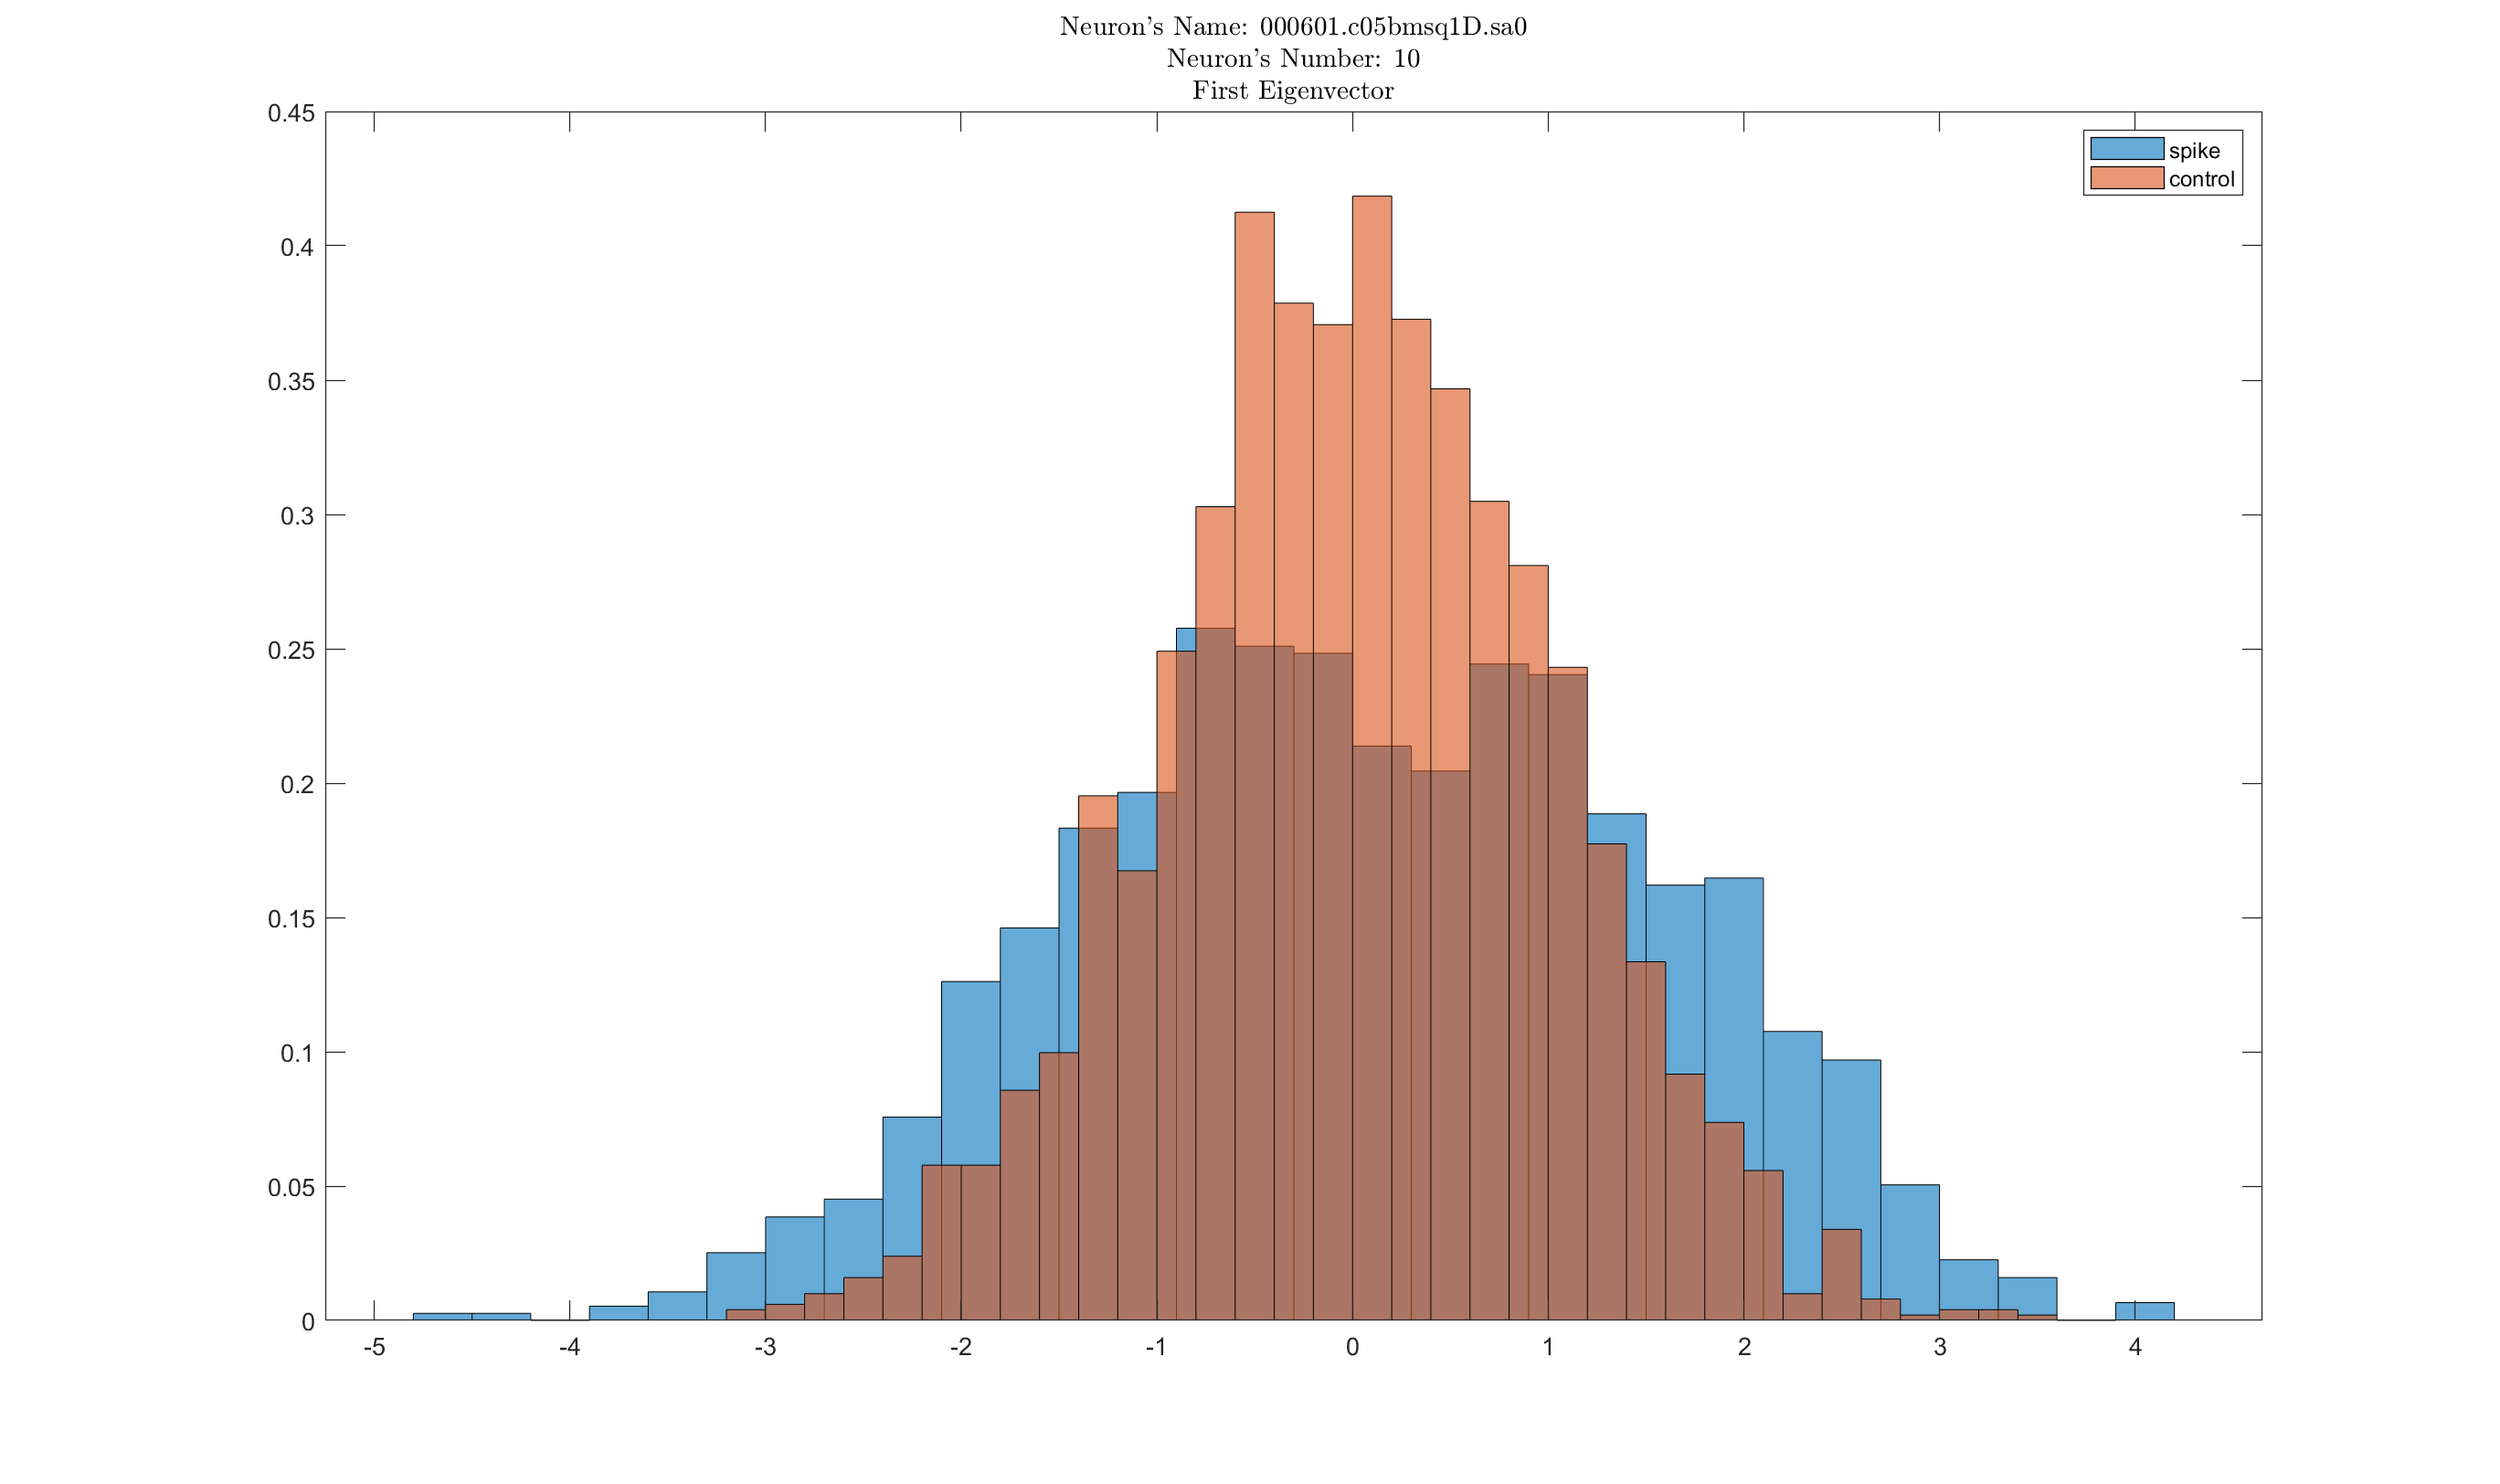
\includegraphics[width=0.45\linewidth]{photos/4_4_First_Eigenvector.png}}
	\subfigure[تصویر تحریک‌ها بر بردار ویژه‌ی دوم]{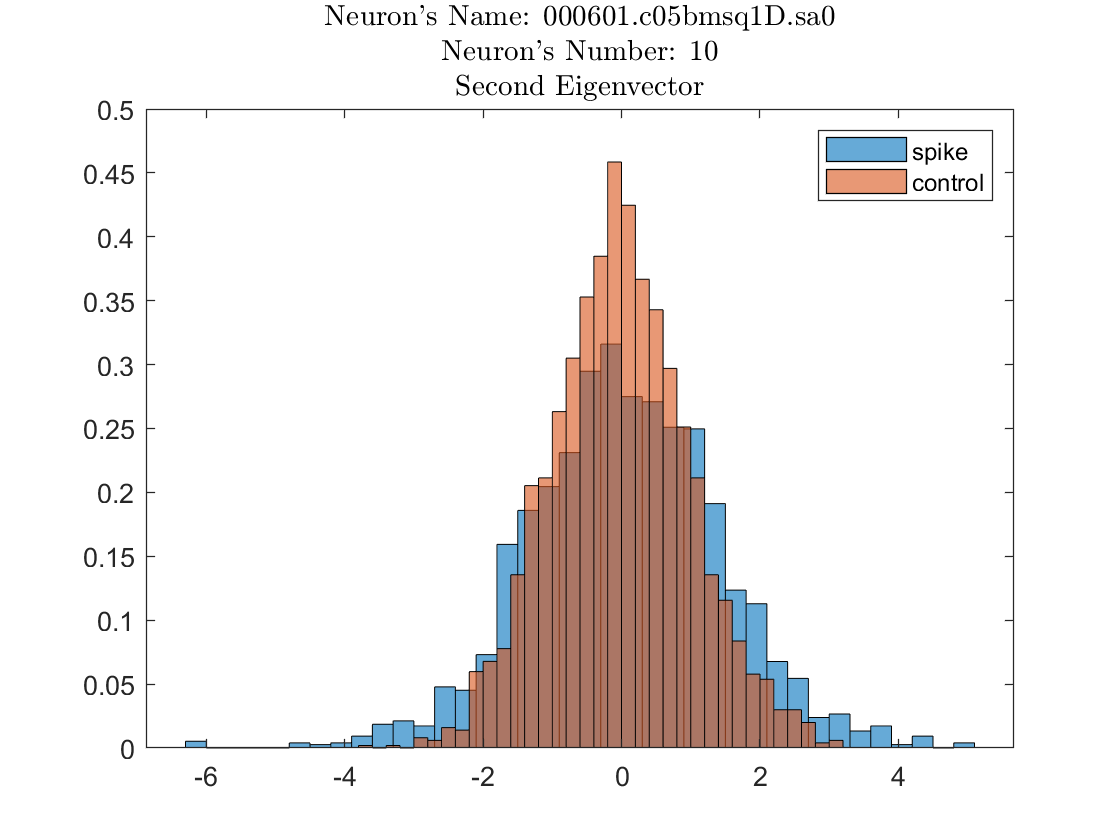
\includegraphics[width=0.45\linewidth]{photos/4_4_Second_Eigenvector.png}}
	\subfigure[توزیع مشترک تصویر‌ها]{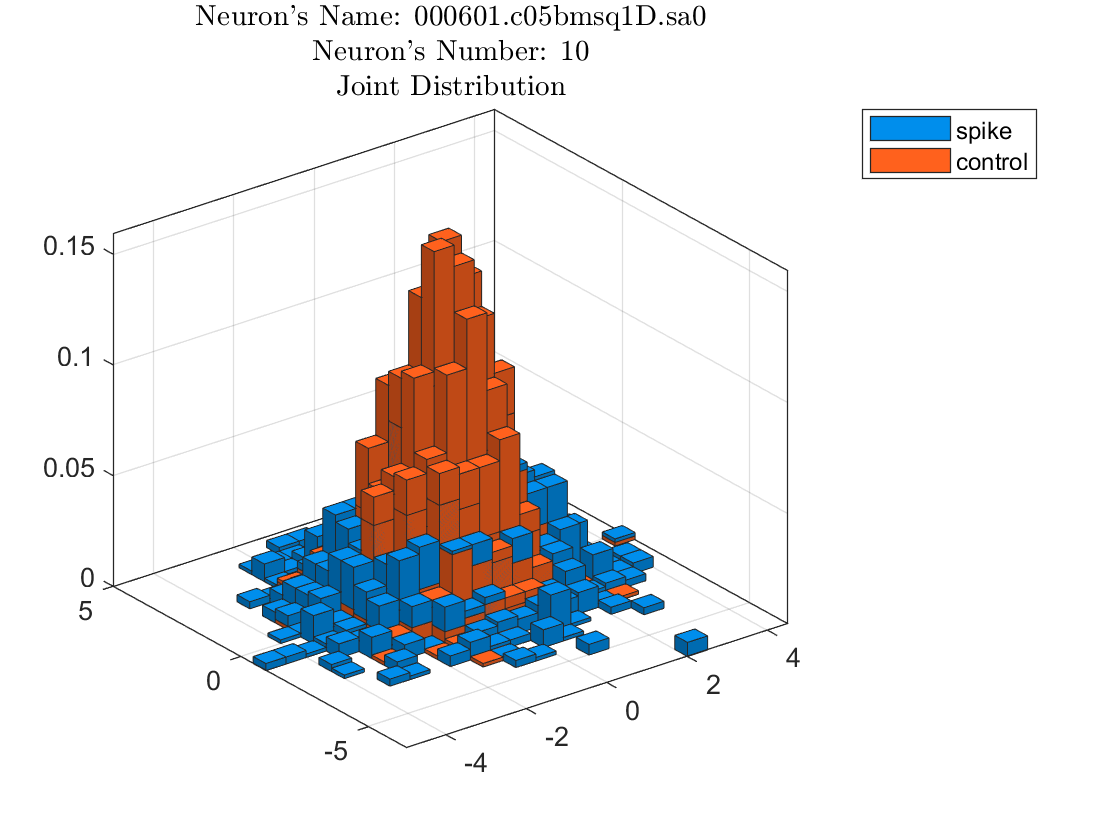
\includegraphics[width=0.6\linewidth]{photos/4_4_3Dhistogram.png}}
\end{figure}

هیستوگرام های فوق، از نظر مفهومی مشابه هیستوگرام موجود در بخش 3-3 هستند. ابتدا هیستوگرام دوبعدی را در نظر بگیرید. در این شکل، دو توزیع به صورت همزمان رسم شده است که یکی مربوط به دادههای تصادفی (\lr{control}) و دیگری مربوط به داده‌های (\lr{spike}) اصلی هستند. این شکل، نشان می دهد که این دو توزیع چه وضعیت نسبت به هم دارند. محورهای افقی، در واقع راستاهای $ v1 $ و $ v2 $ هستند که تحریک های منجر به اسپایک و تحریک‌های تصادفی روی این دو راستا تصویر شده‌اند و این نمودار را تشکیل داده‌اند. مفهوم رسم این دو نمودار روی یک تصویر و مقایسه‌ی آن‌ها، این است که وضعیت یک تحریک، نسبت به این دو راستا چگونه باشد تا منجر به اسپایک بشود، یا نشود. به عنوان نمونه، میبینید که قلهی هیستوگرام نارنجی رنگ (\lr{control}) تقریبا در نقطه (0,0) واقع است. با توجه به این که در حقیقت، مقادیر روی محورها، حاصل ضرب داخلی تحریک در $ v1 $ و $ v2 $ هستند. نقطه (0,0) راستایی را نشان می دهد که هم بر $ v1 $ و هم بر $ v2 $ عمود است. می بینیم که در چنین راستایی، اختلاف تحریک‌های منجر به اسپایک و تحریک‌های تصادفی تقریبا به ماکزیمم خود میرسد و این یعنی اگر یک تحریک نامشخص در این نقطه داشته باشیم، با احتمال بسیار زیاد، منجر به اسپایک نیست و احتمال بیشتری دارد که جزء هیستوگرام نارنجی باشد تا هیستوگرام آبی. به همین ترتیب، در هر نقطه دلخواه از این هیستوگرام سه‌بعدی، میتوان وضعیت دو توزیع منجر به اسپایک و غیرمنجر به اسپایک را مشاهده کرد و آن ها را مقایسه نمود.

دو هیستوگرام دو بعدی دیگر که در بالای هیستوگرام سه بعدی مشاهده می کنید، یکی مربوط به تصویر تحریک‌های منجر، و غیرمنجر به اسپایک روی $ v1 $ و دیگری بر روی $ v2 $‌ است. به تعبیری، این دو هیستوگرام، همان شکل سه بعدی هستند که روی یکی از بعدهای خود جمع شده (انتگرال گرفته شده) است. مفهوم این دو هیستوگرام نیز مشابه بخش 3-3 است، یعنی مقایسه ارتباط تحریک‌های منجر به اسپایک و تحریک‌های غیرمنجر به اسپایک با راستای $ v2 $ و $ v3 $، که هر چقدر دو نمودار (که بر روی یک شکل رسم شده اند) بیشتر از هم جدا باشند، نشان میدهد که راستای مربوطه، توانایی بیشتری در جداکردن این دو گونه تحریک دارد. این حرف در مورد شکل سه‌بعدی نیز برقرار است و هرچقدر دو هیستوگرام سه‌بعدی اسپایک و کنترل بیشتر از هم جدا باشند، میتوان گفت که راستاهای $ v1 $ و $ v2 $، در کنار هم، به شکل مناسب‌تری میتوانند تحریک‌ها را جدا کنند و میتوانیم با داشتن تحریک و این دو راستا، در مورد .اسپایک زدن یا نزدن در اثر آن تحریک صحبت کنیم.
بنابراین، دیدیم که مفهوم این کار با بخش ۳-۳ و عملی که برای \lr{STA} انجام دادیم، کاملا مشابه است. تفاوت این دو بخش آن جاست که در قسمت ۳-۳، ما یک راستا را به عنوان راستای تصمیم‌گیرنده انتخاب کردیم که همان راستای \lr{STA} بود؛ اما در این بخش، ادعا ،می کنیم که یک راستا به تنهایی نمیتواند همه اطلاعات را در بر بگیرد و چند (دو) راستا، میتوانند این عمل را انجام بدهند و بنابراین،د اده‌ها را در دو راستا تصویر میکنیم و به مقایسه تحریک‌های منجر به اسپایک و تحریک‌های بی‌ا‌ثر می‌پردازیم. 

\subsection{بخش پنجم}

بخش عمده‌ی جواب این سؤال را میتوانید در توضیحات مربوط به سؤال قبل جستجو کنید. در واقع، مطابق با توضیحات که در بخش قبل دادیم، میخواهیم روشی انتخاب کنیم که با داشتن یک تحریک نامشخص، تصمیم بگیریم که آیا این تحریک منجر به اسپایک میشود یا نه. برای این کار به هیستوگرام دو بعدی بخش قبل مراجعه میکنیم. تحریک داده شده را روی دو (یا چند) راستای معنی‌دار تصویر میکنیم. فرض کنید دو راستای معنی‌دار داشته باشیم. در این صورت تصویر آن روی $ v1 $ و $ v2 $، دوتایی مرتبی مثل ($ z1 $,$ z2 $) به ما می‌دهد. باید ببینیم که در نقطه متناظر ($ z1 $,$ z2 $) در هیستوگرام بخش قبل، کدام یک از دو دسته‌ی \lr{spike} یا \lr{control} مقادیر بیشتری داشته‌اند. فرض کنید که تحریک‌های منجر به اسپایک در این نقطه مقدار بیشتری دارند. در این صورت میتوانیم بگوییم احتمال آن که چنین تحریکی منجر به اسپایک شود، بیشتر از آن است که منجر به اسپایک نشود. بنابراین تصمیم گیری خود را بر مبنای این احتمال گذاشته و به عنوان جواب نهایی، اعلام میکنیم که این تحریک منجر به اسپایک میشود. حال، با توجه به این توضیحات، واضح است. که برای آن که یک ملاک کلی برای تشخیص اسپایک بیابیم، باید تلافی دو منحنی را حساب کنیم که با فرض گوسی بودن هر دو، میتوانیم با داشتن میانگین و واریانس و ضریب همبستگی خطی مربوط به هر دو توزیع، محل تلاقی آنها را حساب کنیم و شرط اسپایک زدن را اعلام نماییم.
برای آن که ببینیم این روش چقدر موفق عمل کرده، باید ببینیم چند درصد از تحریک هایی که منجر به اسپایک شده اند را به درستی تشخیص میدهد. برای این کار، میتوان همان‌‌طور که گفته شد، محل تلاقی دو توزیع را پیدا کرد.
برای نورون در نظر گرفته شده ، با توجه به روش فوق، نتیجه به شکل زیر است.

\begin{latin}
	\begin{figure}[ht]
			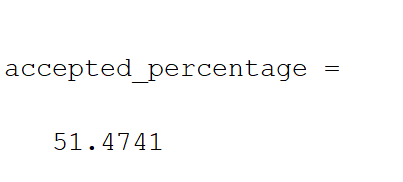
\includegraphics[width=0.35\linewidth]{photos/4_5.png}
	\end{figure}
\end{latin}

\subsection{بخش ششم}
در این بخش با تکرار مراحل ۱ تا ۵ خروجی‌ها را بدست آورده و ذخیره کردیم.

\setcounter{int}{1}
\loop

\begin{figure}[ht]
	\centering
	\includegraphics[trim= 5cm 0 5cm 0, clip= true ,width=0.9\linewidth]{photos/STC/\theint.png}
\end{figure}

\addtocounter{int}{1}\ifnum\value{int}<10
\repeat


\loop

\begin{figure}[ht]
	\centering
	\includegraphics[trim= 5cm 0 5cm 0, clip= true, width=0.9\linewidth]{photos/STC/\theint.png}
\end{figure}


\addtocounter{int}{1}\ifnum\value{int}<18
\repeat

\clearpage

\loop

\begin{figure}[ht]
	\centering
	\includegraphics[trim= 5cm 0 5cm 0, clip= true, width=0.9\linewidth]{photos/STC/\theint.png}
\end{figure}	     


\addtocounter{int}{1}\ifnum\value{int}<55
\repeat 

\clearpage

\subsection{بخش هفتم}
با بررسی جدول قسمت قبل، می بینیم که تقریبا تمامی بردار ویژههای اول، عمده بردار ویژه های دوم و اندکی از بردارویژه‌های سوم ، دارای پترن های معنیدار هستند. این میتواند در مقایسه با \lr{STA} یک پیشرفت محسوب شود، چرا که در \lr{STA} ، بسیاری از \lr{receptive field} های بدست آمده، فاقد پترن معنی دار بودند.
امّا سؤال مهم تر این است که آیا در تمامی موارد توانستهایم بهتر از روش کلاسیک عمل کنیم یا نه؟ ابتدا به درصدهای موجود در جدول بخش قبل مراجعه میکنیم. آنچه در جدول می بینیم کاملا خلاف انتظار ماست. اولاً که تعداد زیادی درصد کمتر از ۵۰ مشاهده میکنیم (که در روش کلاسیک چنین نبود) و این به آن معناست که سنجش ما دارد ضعیفتر از حالت رندوم عمل میکند. یعنی اگر تحریکها را به صورت تصادفی به دو دسته موثر و بیاثر تقسیم میکردیم، نتیجهی بهتری از این دستهبندی میگرفتیم. البته در این گونه مسائل دستهبندی، نتیجهی بسیار بد، مانند روی دیگری از یک سکه است که در طرف دیگر آن، نتیجه‌ی بسیار خوب قرار دارد. یعنی اگر به عنوان مثال، ما در ۲۰ درصد موارد بتوانیم جواب درست را تشخیص دهیم (با توجه به این که جواب، دو حالت دارد؛ اسپایک زدن یا نزدن) میتوانیم صرفاً جوابمان را در تمامی حالات عوض کنیم. به این ترتیب، در ۸۰ درصد موارد ، جواب درست می دهیم. با این وجود، ما انتظار داریم که پس از حجم زیادی از تحلیل و محاسبات، درصد تحریکهایی که به درستی تشخیص داده میشوند، با اختلاف بالای 50 باشند که در عمل، مشاهده کردیم که چنین نشد. در واقع، دیدیم که در بسیاری از موارد گویی \lr{STA} بهتر پاسخ می دهد تا
\lr{STC}
(\lr{Spike-Triggered Correlation}).

\pagebreak

\section{طرح سوال‌ دلخواه}
\subsection{صورت مسئله‌ی طرح شده}
با خواندن مقاله متوجه می‌شویم که هدف آن یافتن راستا‌هاییست که در آن داده‌های موجب اسپایک، واریانس به طور قابل‌ توجه زیادتری نسبت به کل داده‌ها داشته باشد و در نتیجه توزیع داده‌های موجب اسپایک در آن راستا با توزیع کل داده‌ها متفاوت باشد. در طول انجام این پروژه به این موضوع اشاره نشد. 

در اینجا می‌خواهیم این موضوع را مشاهده کنیم یعنی اولاً ببینیم که در راستاهای پیشنهادی مقالی واریانس داده‌ها به طرز قابل توجهی بیشتر از کل داده‌هاست و ببینیم که در روش کلاسیک \lr{STA} این موضوع برقرار نیست. ثانیاً با بررسی بردارویژه‌های مرتب شده نوع تغییر \lr{p-value} در تست واریانس را ببینیم.


\subsection{تست مورد استفاده}
برای بررسی موضوعات گفته شده به یک تست آماری نیاز داریم که بزرگ‌تر بودن واریانس یک نمونه‌ نسبت به یک نمونه‌ی دیگر را بررسی کند. با جست‌وجو برای این هدف به تست \lr{f-test} دست پیدا کردیم که تابع آماده آن موجود است به طور کلی \lr{f-test} برای دو جمعیت استفاده می‌شود تا ببینیم آیا این دو جمعیت واریانس یکسانی دارند یا نه. ما در اینجا می‌خواهیم از آزمون یک-طرفه استفاده کنیم و تنها بزرگ‌تر بودن واریانس جمعیت اول(توزیع‌ تحریک‌ها به شرط اسپایک) را بررسی کنیم بنابراین:

\begin{latin}
\begin{itemize}
	\item 
	$H_0:$ \space $\sigma_1^2 = \sigma_2^2$
	\item 
	$H_a:$ \space
	$\sigma_1^2 > \sigma_2^2$
\end{itemize}
\end{latin}

\subsection{رویکرد و نتایج به دست آمده}
رویکردی که در پیش می‌گیریم این است که ابتدا تصویر توزیع‌ها در راستای‌ \lr{STA}
و بردارویژه‌ی اصلی بدست آمده در روش \lr{STC} را ملاک قرار می‌دهیم و برای تمامی نورون‌ها آزمایش \lr{f-test} را انجام می‌دهیم نهایتا می‌خواهیم درصد رد شدن فرض صفر به ازای همه‌ی نورون‌ها و برای هر رویکرد بررسی کنیم. کلیت کار مشابه قبل خواهد بود و تنها تستی که می‌گیریم متفاوت است. خروجی به صورت زیر خواهد بود:

\begin{latin}
	\begin{lstlisting}[basicstyle=\small, frame = single]
mean result for Spike triggered correlation:1
mean result for Spike triggered correlation:6.481481e-01
	\end{lstlisting}
\end{latin}

مشاهده می‌کنیم که برای \lr{STC} با درصد بسیار خوبی ۱۰۰ درصد تمامی فرض صفر‌ها را رد کردیم به عبارت دیگر برای تمامی نورون‌ها توزیع تحریک به شرط وجود اسپایک با توزیع تحریک در راستای‌ مقدارویژه‌ی اصلی که برای ماتریس \lr{STC} به دست می‌آوریم به لحاظ واریانس اختلاف قابل توجهی دارد که این موضوع برای \lr{STA} صدق نمی‌کند.

در بخش بعد برای نورون با کد
 \lr{020321.A.i}
 و برای تمامی بردارویژه‌هایی که از روش \lr{STC} به دست آوردیم مراحل تست را تکرار می‌کنیم، اینجا پرسش ما این است که آیا \lr{p-value}ها ادعای مقاله مبنی بر بی‌اثر بودن تعداد زیاد از ویژگی‌ها را تایید می‌کند یا خیر. خروجی به دست آمده از اجرای کد نمودار زیر خواهد بود.
 
 \begin{figure}[ht]
 	\centering
 	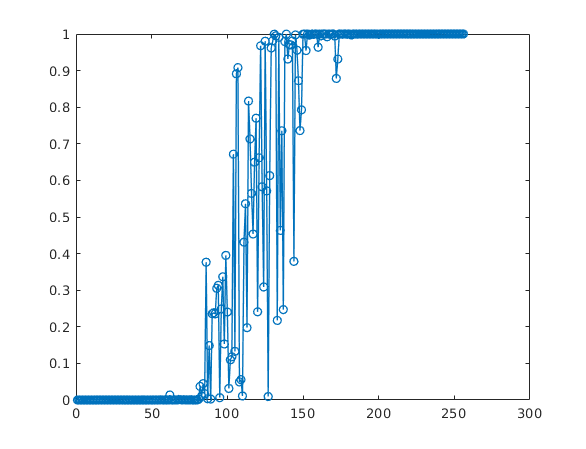
\includegraphics[width=0.6\linewidth]{photos/p-value-eigenvectors.png}
 	\caption{\lr{p-value}
 	ها برای بردار‌ویژه‌های بزرگ‌تر تا کوچک‌تر	
 }
 \end{figure}	     

همانطور که می‌توان دید برای بسیاری از نورون‌ها \lr{p-value} مقدار یک را دارد که این نشان می‌دهد آن بردارویژه‌ها با احتمال بسیار بالایی به هیچ‌وجه در تغییر واریانس و در نتیجه تغییر توزیع قبل و پس از دیدن پاسخ نورون ندارند.

\end{document}